\documentclass[11pt,a4paper]{ctexart}

\title{物理必修\ 第二册}
\author{啊波呲}

\setlength{\parskip}{0em}
\usepackage{amsmath,mathtools,amssymb,geometry,wrapfig,graphicx,empheq,pifont}
\renewcommand{\baselinestretch}{1.8}
\geometry{left=1.5cm,right=1.5cm,bottom=2cm,top=2.5cm}
\usepackage{tikz}
\usepackage{xcolor}
\newcounter{exam}[section]
\setcounter{exam}{0}
\begin{document}
\maketitle
\pagenumbering{roman}
\tableofcontents

\newpage
\pagenumbering{arabic}

\section{运动的合成与分解}

\subsection{曲线运动}

运动轨迹是曲线(非直线)的运动称为\textbf{曲线运动}.

\subsubsection*{物体做曲线运动的条件}

实验表明,当加速度的方向与速度的方向不在同一直线上时,物体做曲线运动.

从另一个角度来说,当合力的方向与速度的方向不在同一直线上时,物体做曲线运动.

\subsubsection*{曲线运动的特点}
\begin{enumerate}
	\item 质点做曲线运动,其某一时刻速度的方向,沿曲线在这一点的\textbf{切线}方向.
	\item 物体做曲线运动时,速度的方向时刻都在改变,所以物体的加速度一定不为0;但速度的大小(即速率)可能不变.
	\item 物体做曲线运动的轨迹一定夹在合力方向(或加速度方向)与速度方向之间.
	\item 做曲线运动的物体, 当合力方向(或加速度方向)与速度速度方向的夹角为锐角时,物体的速率将增大;
	      当合力方向(或加速度方向)与速度速度方向的夹角为钝角时,物体的速率将减小.
	\item 做曲线运动的物体, 位移小于路程.
\end{enumerate}

加速度恒定的曲线运动叫做\textbf{匀变速曲线运动}.

\subsubsection*{曲线运动的轨迹}

简单来说, 当物体的初速度与所受的 (恒定的) 合力不在一条直线上时, 物体起初会向初速度的方向运动, 但轨迹会向合力的方向逐渐偏移,
形成曲线. 需要注意的是, \textbf{物体的运动方向永远不会和合力的方向平行}.

\subsection{运动的合成与分解}

与合力,分力的概念类似, 如果一个物体同时参与了几个不同方向上的运动,
那么这几个运动都叫做该物体实际运动的\textbf{分运动},
该物体的实际运动叫做这几个运动的\textbf{合运动}.

运动的合成与分解遵循矢量的平行四边形法则.

\subsubsection*{合运动类型的判断}

\setlength{\abovedisplayskip}{3pt}
\setlength{\belowdisplayskip}{3pt}

\begin{enumerate}
	\item 两个匀速直线运动的合运动是匀速直线运动;
	\item 一个匀速直线运动和一个匀加速直线运动做合成, 当这两个分运动共线时,
	      合运动是匀变速直线运动;当这两个分运动不共线时,合运动是匀变速曲线运动.
	\item 两个匀变速直线运动的合运动,可能是匀变速直线运动,也可能是匀变速曲线运动.\\
	      事实上,当这两个分运动的速度$v_1$, $v_2$,加速度$a_1$, $a_2$对应成比例时,即满足
	      $$\frac{v_1}{v_2}=\frac{a_1}{a_2}$$
	      时,物体做匀变速直线运动;否则,物体做匀变速曲线运动.

\end{enumerate}

\subsection{小船过河问题}

小船在过流动的河时,实际上参与了两个方向的分运动,即随水流的运动和船相对于水的运动(可看作船在静水中的运动).

\subsubsection*{最短时间问题}

\begin{wrapfigure}{r}{4cm}
	\flushright
	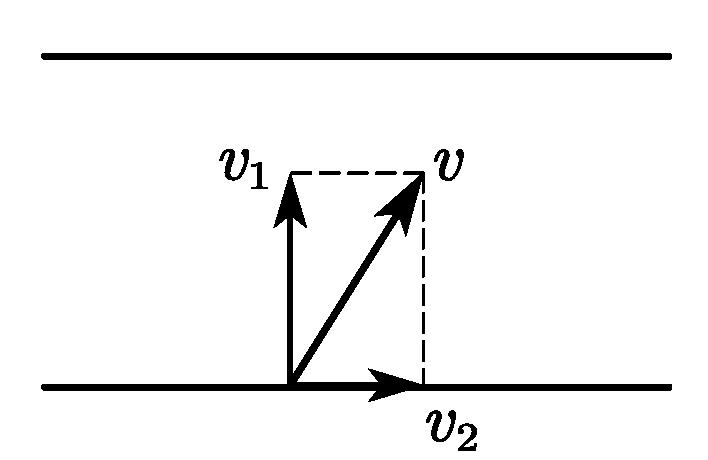
\includegraphics[width=0.25\textwidth]{pic/pic5.pdf}
	\label{fig5}
\end{wrapfigure}

小船过河的时间,是由垂直于河岸的分运动决定的.因此,为使渡河时间最短,应让小船垂直于河岸的分速度最大.
于是小船应该垂直于河岸行驶.

如右图, 河宽为$d$, 船在静水中的速度为$v_1$, 水流的速度恒为$v_2$, 它们的合速度为$v$.

船在静水中的速度$v_1$即为小船垂直于河岸的分速度, 此时的过河时间$$t = \frac{d}{v_1}.$$

小船垂直于河岸的分运动与沿水流方向的分运动均为匀速直线运动, 我们知道, 小船的实际运动也是匀速直线运动,
并且轨迹就是物体的合运动$v$所在的直线.小船的位移
$$s=vt=\sqrt{{v_1}^2 + {v_2}^2}\ t = \frac{d\sqrt{{v_1}^2 + {v_2}^2}}{v_1}.$$

\subsubsection*{最短位移问题}

小船过河的运动可以分解为平行于河岸和垂直于河岸两个方向的分运动.

因为在渡河时, 垂直于河岸方向的分位移恒为河宽$d$, 所以要使渡河位移最短, 只需控制平行于河岸方向的分位移最小.

\begin{wrapfigure}{r}{4cm}
	\flushright
	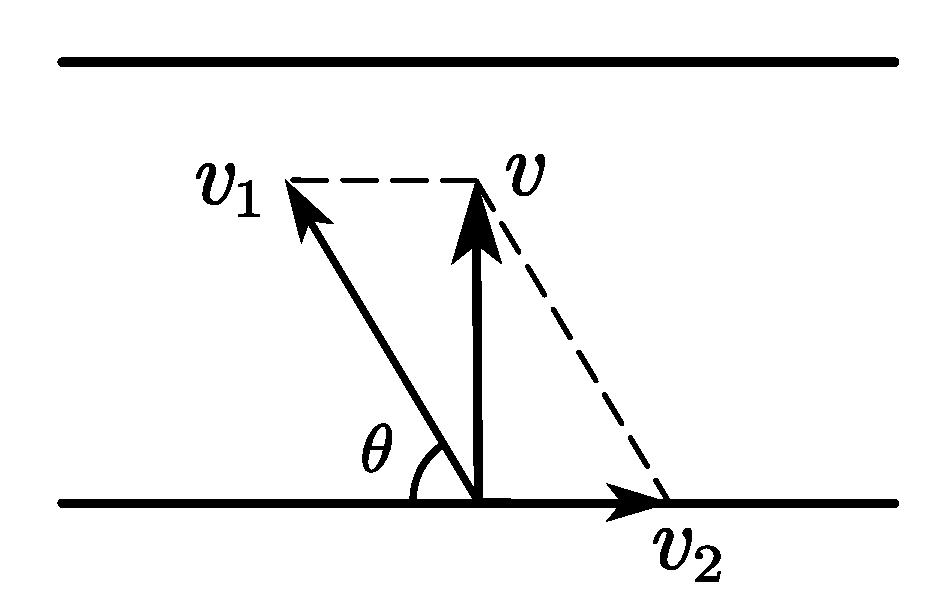
\includegraphics[width=0.25\textwidth]{pic/pic6.pdf}
	\label{fig6}
\end{wrapfigure}

若平行于河岸方向的分位移为0, 即小船实际运动垂直于河岸, 则船速$v_1$在平行于河岸方向上须与水速$v_2$等大反向.
因此, 应将船头偏向上游, 并与河岸成一定的角度$\theta$, 如右图所示.
\setlength{\abovedisplayskip}{3pt}
\setlength{\belowdisplayskip}{3pt}

根据几何关系,有 $$v_1 \cos{\theta} - v_2 = 0.$$
因为$\cos \theta \in [0,1]$,所以只有在船速$v_1$大于水速$v_2$时,小船的实际位移才有可能垂直于河岸.
因此,需要分两种情况讨论.

当$v_1 > v_2$时, 应使船速$v_1$与水速$v_2$的合速度$v$与河岸垂直, 如上图所示 .此时船速 $v_1$
方向与河岸方向的夹角$\theta$满足$$\cos{\theta} = \frac{v_1}{v_2}.$$最小位移就是河宽$d$.
合速度的大小$$v = v_1 \sin{\theta}.$$
对应的渡河时间$$t = \frac{d}{v} = \frac{d}{v_1 \sin{\theta}}.$$

\begin{wrapfigure}{r}{4cm}
	\flushright
	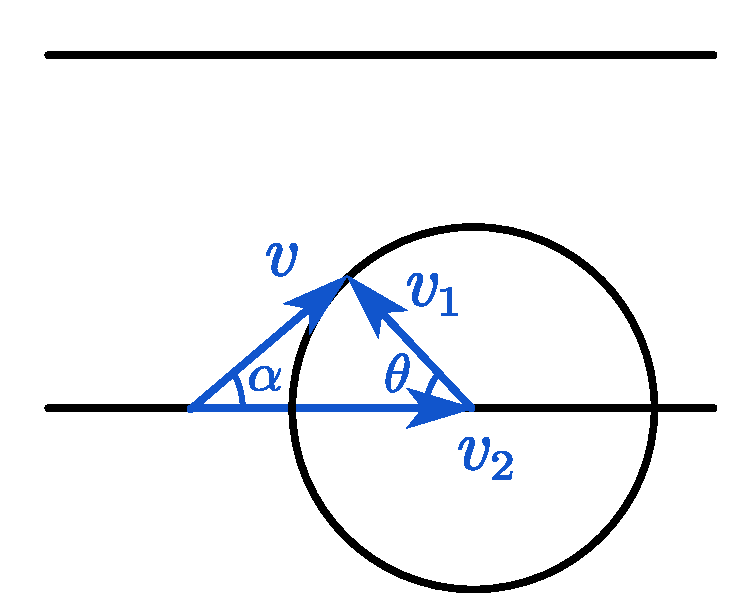
\includegraphics[width=0.25\textwidth]{pic/pic7.pdf}
	\label{fig6}
\end{wrapfigure}

(2) 当$v_1 < v_2$时, 由于水流的冲击,小船是无法沿垂直于河岸的方向运动的. 此时合速度$v$指向下游,
与河岸的夹角为$\alpha$.由几何关系可知,渡河位移$$s = \frac{d}{\sin {\alpha}}.$$
显然, 当$\alpha \in [0,\pi]$时, $s$随角$\alpha$的增大而减小.

如右图所示, 以水速矢量$v_2$的终点为圆心, 以船速矢量$v_1$的大小为半径作圆. 从水速矢量$v_2$的起点向圆作切线,
切点为合速度矢量$v$的终点. 显然, 沿此方向的航程是最短的.

由几何关系可知, 当位移最短时, 船速 $v_1$ 方向与河岸方向的夹角$\theta$满足 $$\cos{\theta} = \frac{v_1}{v_2}.$$
此时的位移 $$s = \frac{d}{\sin \left (\displaystyle\frac{\pi}{2}-\theta \right )} = \frac{v_2}{v_1} d.$$

\section{平抛运动}
\subsection{平抛运动的基本概念}

平抛运动是水平抛出的物体只受重力作用时所做的运动.
它是加速度为重力加速度 $g$ 的\textbf{匀变速曲线运动},轨迹是抛物线.

在处理平抛运动的问题时,我们通常\textbf{把平抛运动分解为水平方向的匀速直线运动和竖直方向的自由落体运动}.

\subsubsection{运动规律}

以初速度 $v_0$ 沿水平方向抛出一物体,物体做平抛运动.由于物体只受到竖直向下的重力,
所以它在水平方向上的加速度为 0,竖直方向上的加速度为重力加速度 $g$,那么在整个运动过程中,
物体在水平方向上的速度 $ v_{x}$ 将保持初速度 $v_0$ 恒定不变;而在竖直方向上的速度 $v_y$
满足自由落体的规律.因此,物体在水平方向和竖直方向的分速度与时间 $t$ 的关系分别为
\setlength{\abovedisplayskip}{3pt}
\setlength{\belowdisplayskip}{3pt}
\begin{align*}
	v_x=v_0, \\
	v_y=gt.
\end{align*}
那么物体的合速度
\begin{equation}
	\label{合速度}
	v=\sqrt{{v_x}^2+{v_y}^2}=\sqrt{{v_0}^2+\left(gt\right)^2}.
\end{equation}

因此,物体在$t$时间内的水平位移
\begin{equation}
	\label{水平位移}
	x=v_0t,
\end{equation}
竖直位移
\begin{equation}
	\label{竖直位移}
	y=\frac12gt^2,
\end{equation}
合位移 $$s=\sqrt{x^2+y^2}=\sqrt{\left(v_0t\right)^2+\left(\frac{1}{2}gt^2\right)^2}.$$

\begin{wrapfigure}{r}{7cm}
	\flushright
	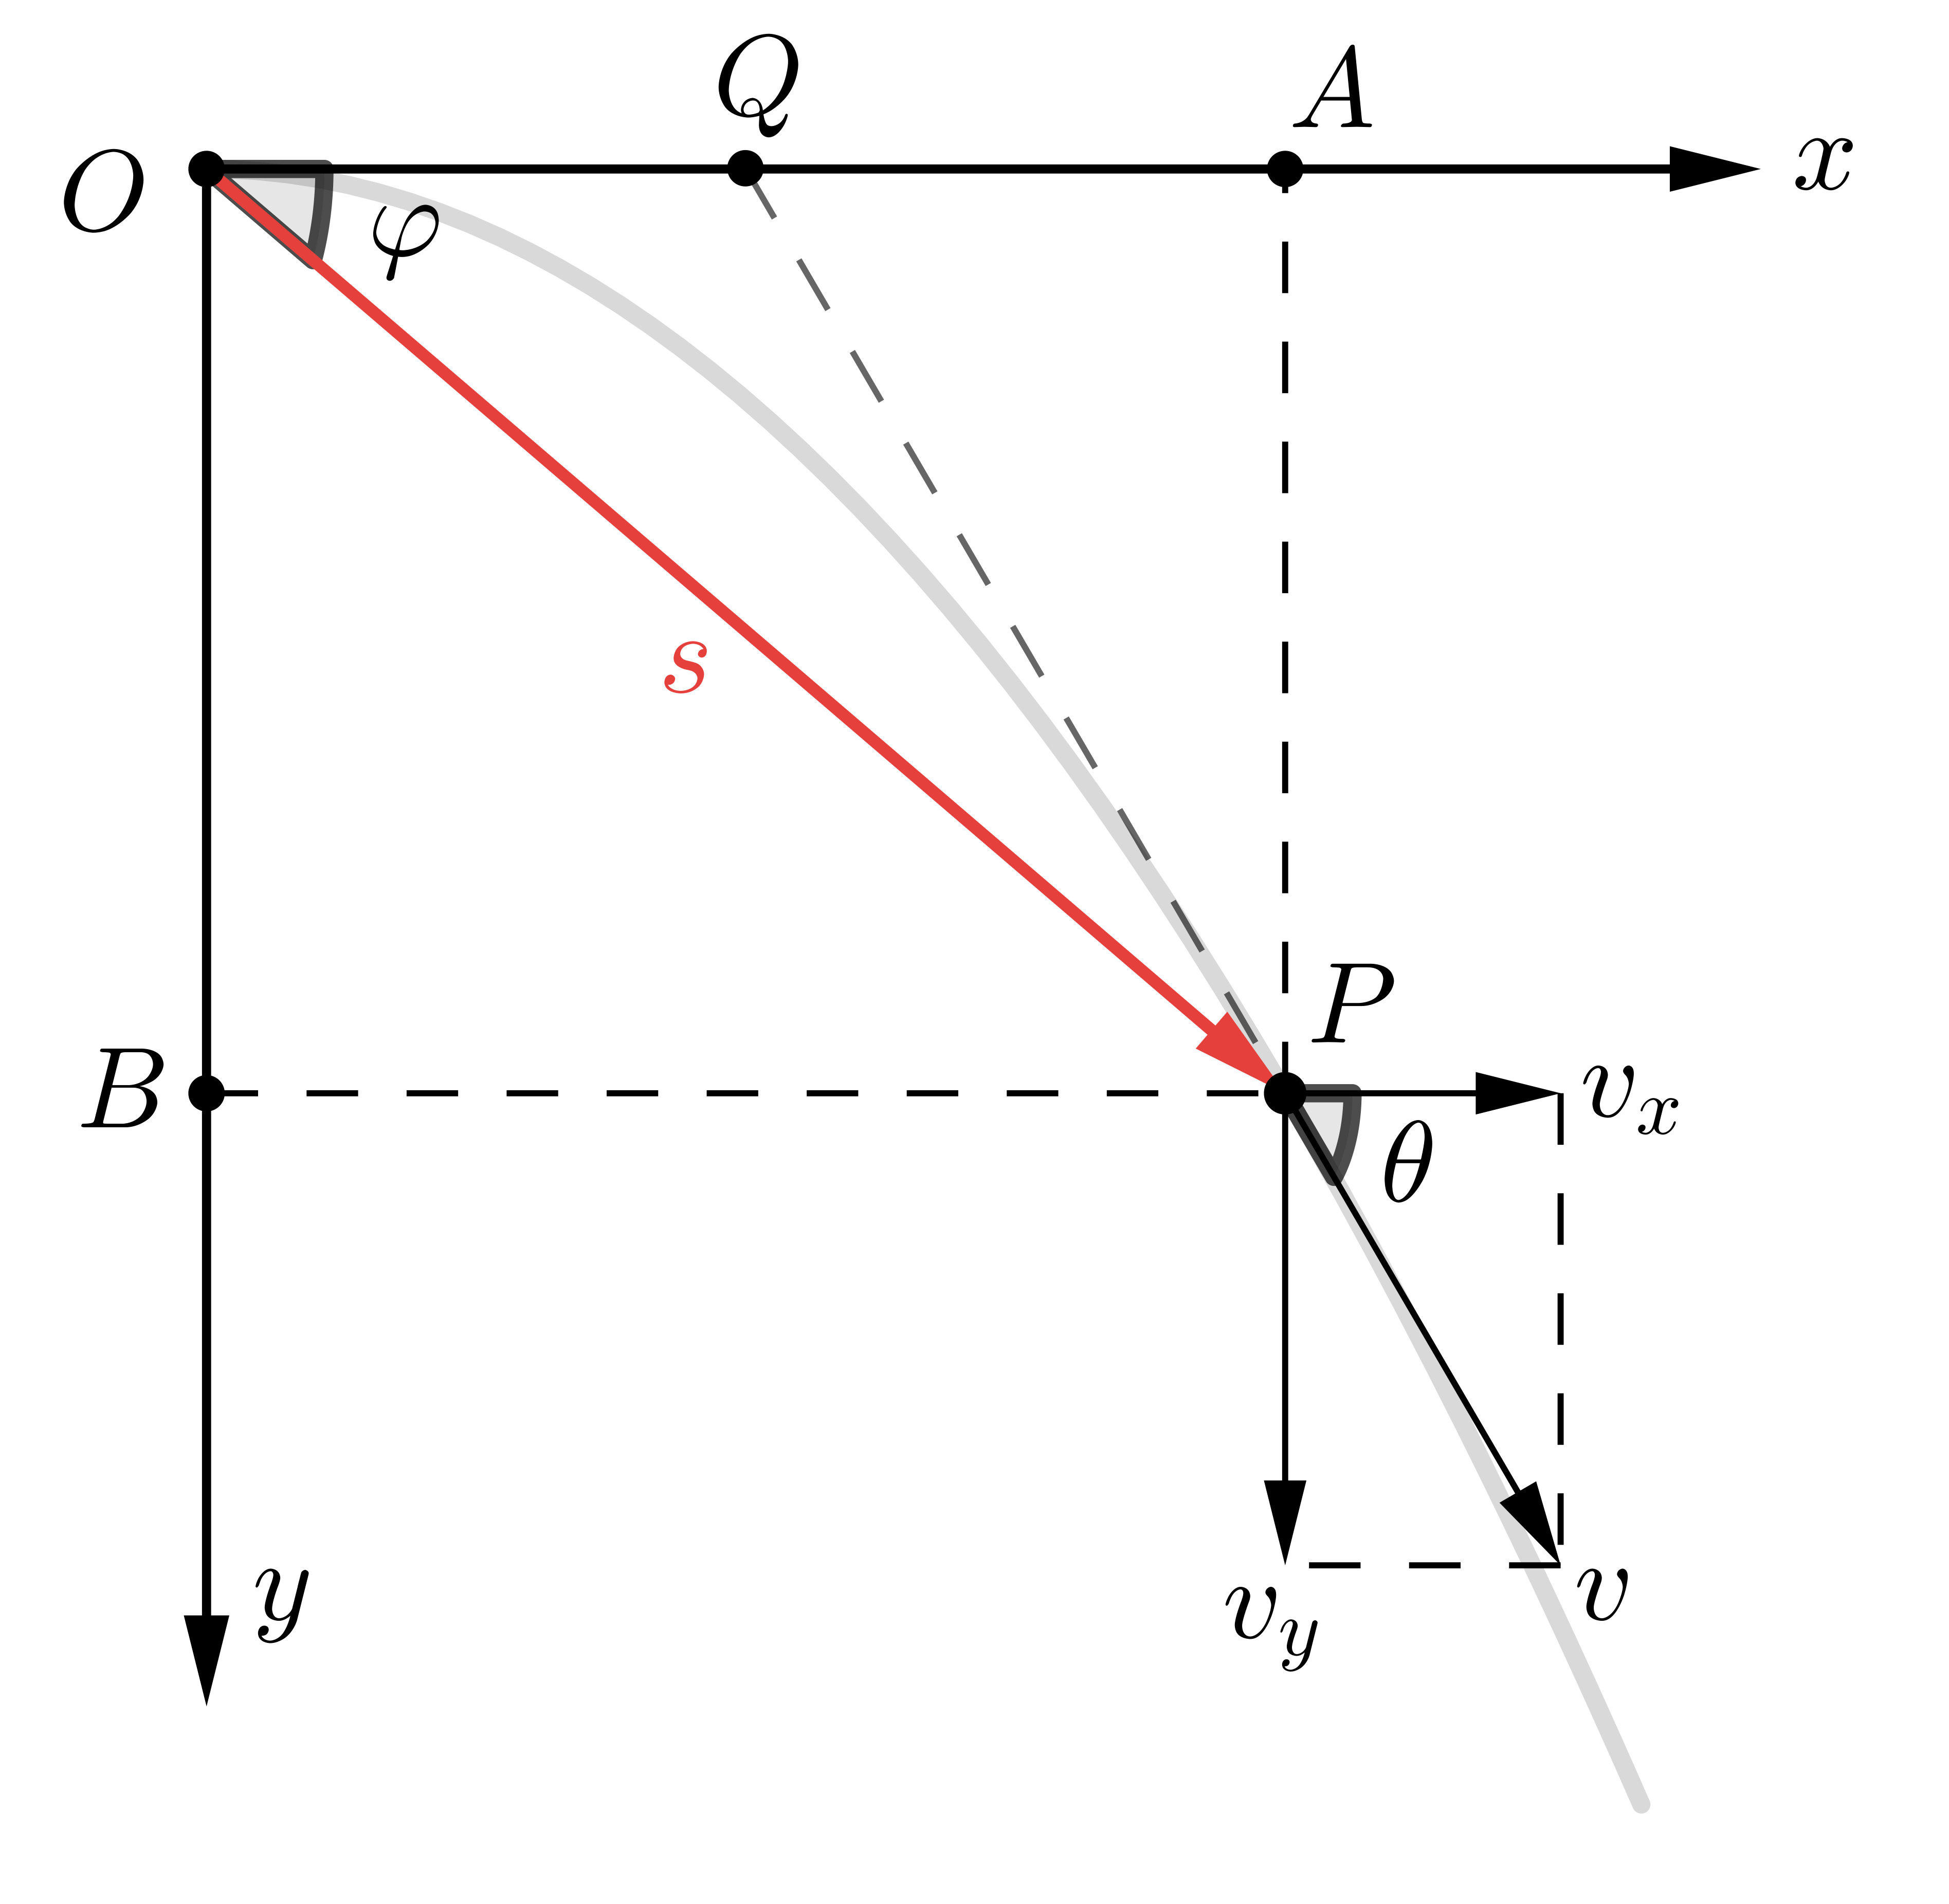
\includegraphics[width=0.38\textwidth]{pic/pic1.png}
	\label{fig1}
\end{wrapfigure}
为便于分析平抛运动的特点,我们以初速度的方向为 $x$ 轴方向,
竖直向下的方向为 $y$ 轴方向,建立直角坐标系(如右图).

联立 \eqref{水平位移}\eqref{竖直位移},消去 $t$,我们有
\begin{empheq}[box=\fbox]{equation}
	\label{平抛运动轨迹方程}
	y=\frac{g}{2{v_0}^2}x^2.
\end{empheq}
(\ref{平抛运动轨迹方程})式叫做\textbf{平抛运动的轨迹方程}.

根据平抛运动的运动规律, 我们有两个推论.

\subparagraph{推论 1}
做平抛运动的物体,设其末速度方向与水平方向的夹角为 $\theta$,
位移方向与水平方向的夹角为 $\varphi$,则在运动过程中恒有
\setlength{\abovedisplayskip}{3pt}
\setlength{\belowdisplayskip}{3pt}
\begin{empheq}[box=\fbox]{equation*}
	\tan{\theta}=2\tan{\varphi}.
\end{empheq}

\textbf{证明}\ \ \
根据几何关系有
\setlength{\abovedisplayskip}{3pt}
\setlength{\belowdisplayskip}{3pt}
$$\tan{\theta}=\frac{v_y}{v_x}=\frac{gt}{v_0}, $$
$$\tan{\varphi}=\frac{y}{x}=\frac{\frac{1}{2}gt^2}{v_0t}=\frac{gt}{2v_0}.$$

于是
$$\tan{\theta}=2\tan{\varphi}.$$

\subparagraph{推论 2}
做平抛运动的物体,任一时刻的瞬时速度的反向延长线过此刻水平位移的中点.
如图,$PQ$ 是速度 $v$ 的反向延长线,有 $OQ=\displaystyle\frac{1}{2}OA$.

\textbf{证明}\ \ \
由(\ref{水平位移})(\ref{竖直位移})式可知
$$\frac{y}{\frac{x}{2}}=\frac{gt}{v_0}=\tan{\theta}=\frac{v_y}{v_x}.$$
可知瞬时速度的反向延长线过此刻水平位移的中点.

\subsubsection{推导公式}

以速度$v_0$从高度$h$处水平抛出一物体,该物体在竖直方向上做自由落体运动,
根据匀变速直线运动位移$h$与时间$t$的关系$h=\displaystyle\frac{1}{2}gt^2$可知,物体做平抛运动的运动时间
\begin{equation}
	\setlength{\abovedisplayskip}{3pt}
	\setlength{\belowdisplayskip}{3pt}
	\label{运动时间}
	t=\sqrt{\frac{2h}{g}}.
\end{equation}
上式告诉我们,\textbf{物体做平抛运动的飞行时间取决于下落的高度}.上式也可以表示为$$t\propto \sqrt{h}.$$

联立(\ref{水平位移})(\ref{运动时间}),消去 $t$,我们就得到物体做平抛运动的水平位移
$$x=v_0\sqrt{\frac{2h}{g}}.$$
上式告诉我们,\textbf{物体做平抛运动的水平位移与初速度和下落高度均有关}.

由于物体在竖直方向上做自由落体运动,根据匀变速直线运动位移 $h$ 与速度 $v_y$ 的关系 $2gh=v_y^2$,
结合(\ref{合速度})式可以得到,物体做平抛运动的落地速度
$$v=\sqrt{{v_0}^2+2gh}.$$
上式告诉我们,\textbf{物体做平抛运动的落地速度与初速度和下落高度均有关}.

因为做平抛运动的物体只受到重力作用,即只具有竖直向下的重力加速度 $g$,
所以该物体在水平方向的分速度 $v_x$ 恒为初速度 $v_0$ 不变,
只有竖直方向的分速度 $v_y$ 每间隔时间 $\Delta t$ 就增加 $g\Delta{t}$,
因此,做平抛运动的物体,在任意两段连续相等的时间间隔内,速度的变化量$\Delta{v}$与时间间隔 $\Delta{t}$ 的关系为
\begin{equation}
	\label{速度变化量与时间间隔的关系}
	\Delta{v}=\Delta{v_y}=g \Delta t.
\end{equation}

做平抛运动的物体,在连续相等的时间间隔内,竖直方向上的位移差 $\Delta{y}$ 与时间间隔 $\Delta t$
的关系为 $\Delta{y}=\Delta{v} \Delta t$,代入(\ref{速度变化量与时间间隔的关系}),得到
$$\Delta{y}=g(\Delta{t})^2.$$
即位移差不变.

\subsubsection{解决简单问题}
\refstepcounter{exam}
\subparagraph{例\theexam}
把一个小球从离地$h=5\ \rm{m}$高度处,以 $v_0=10\ \rm{m/s}$ 的初速度水平抛出,不计空气阻力,
取 $g=10\ \rm{m/s^2}$.求:

(1) 小球在空中飞行的时间;

(2) 小球落地点距离抛出点的水平距离;

(3)小球落地时的速度大小.

\textbf{解}\ \ \ (1)由题意可知,小球做平抛运动,其竖直方向的分运动是自由落体,
根据匀变速直线运动位移$h$与时间 $t$ 的关系有 $$h=\frac12gt^2, $$
所以小球在空中飞行的时间
$$t=\sqrt{\frac{2h}{g}}=\sqrt{\frac{2\times5}{10}}\ \rm{s}=1\ \rm{s}.$$

(2)小球的水平位移 $$x=v_0t=10\ \rm{m/s}\times1\ \rm{s}=10\ \rm{m}.$$

(3)小球落地时的竖直分速度 $$v_y=gt=10\ \rm{m/s}.$$
所以落地时的速度 $$v=\sqrt{{v_x}^2+{v_y}^2}=\sqrt{{v_0}^2+{v_y}^2}=10\sqrt2\ \rm{m/s}.$$

\begin{wrapfigure}{r}{3cm}
	\flushright
	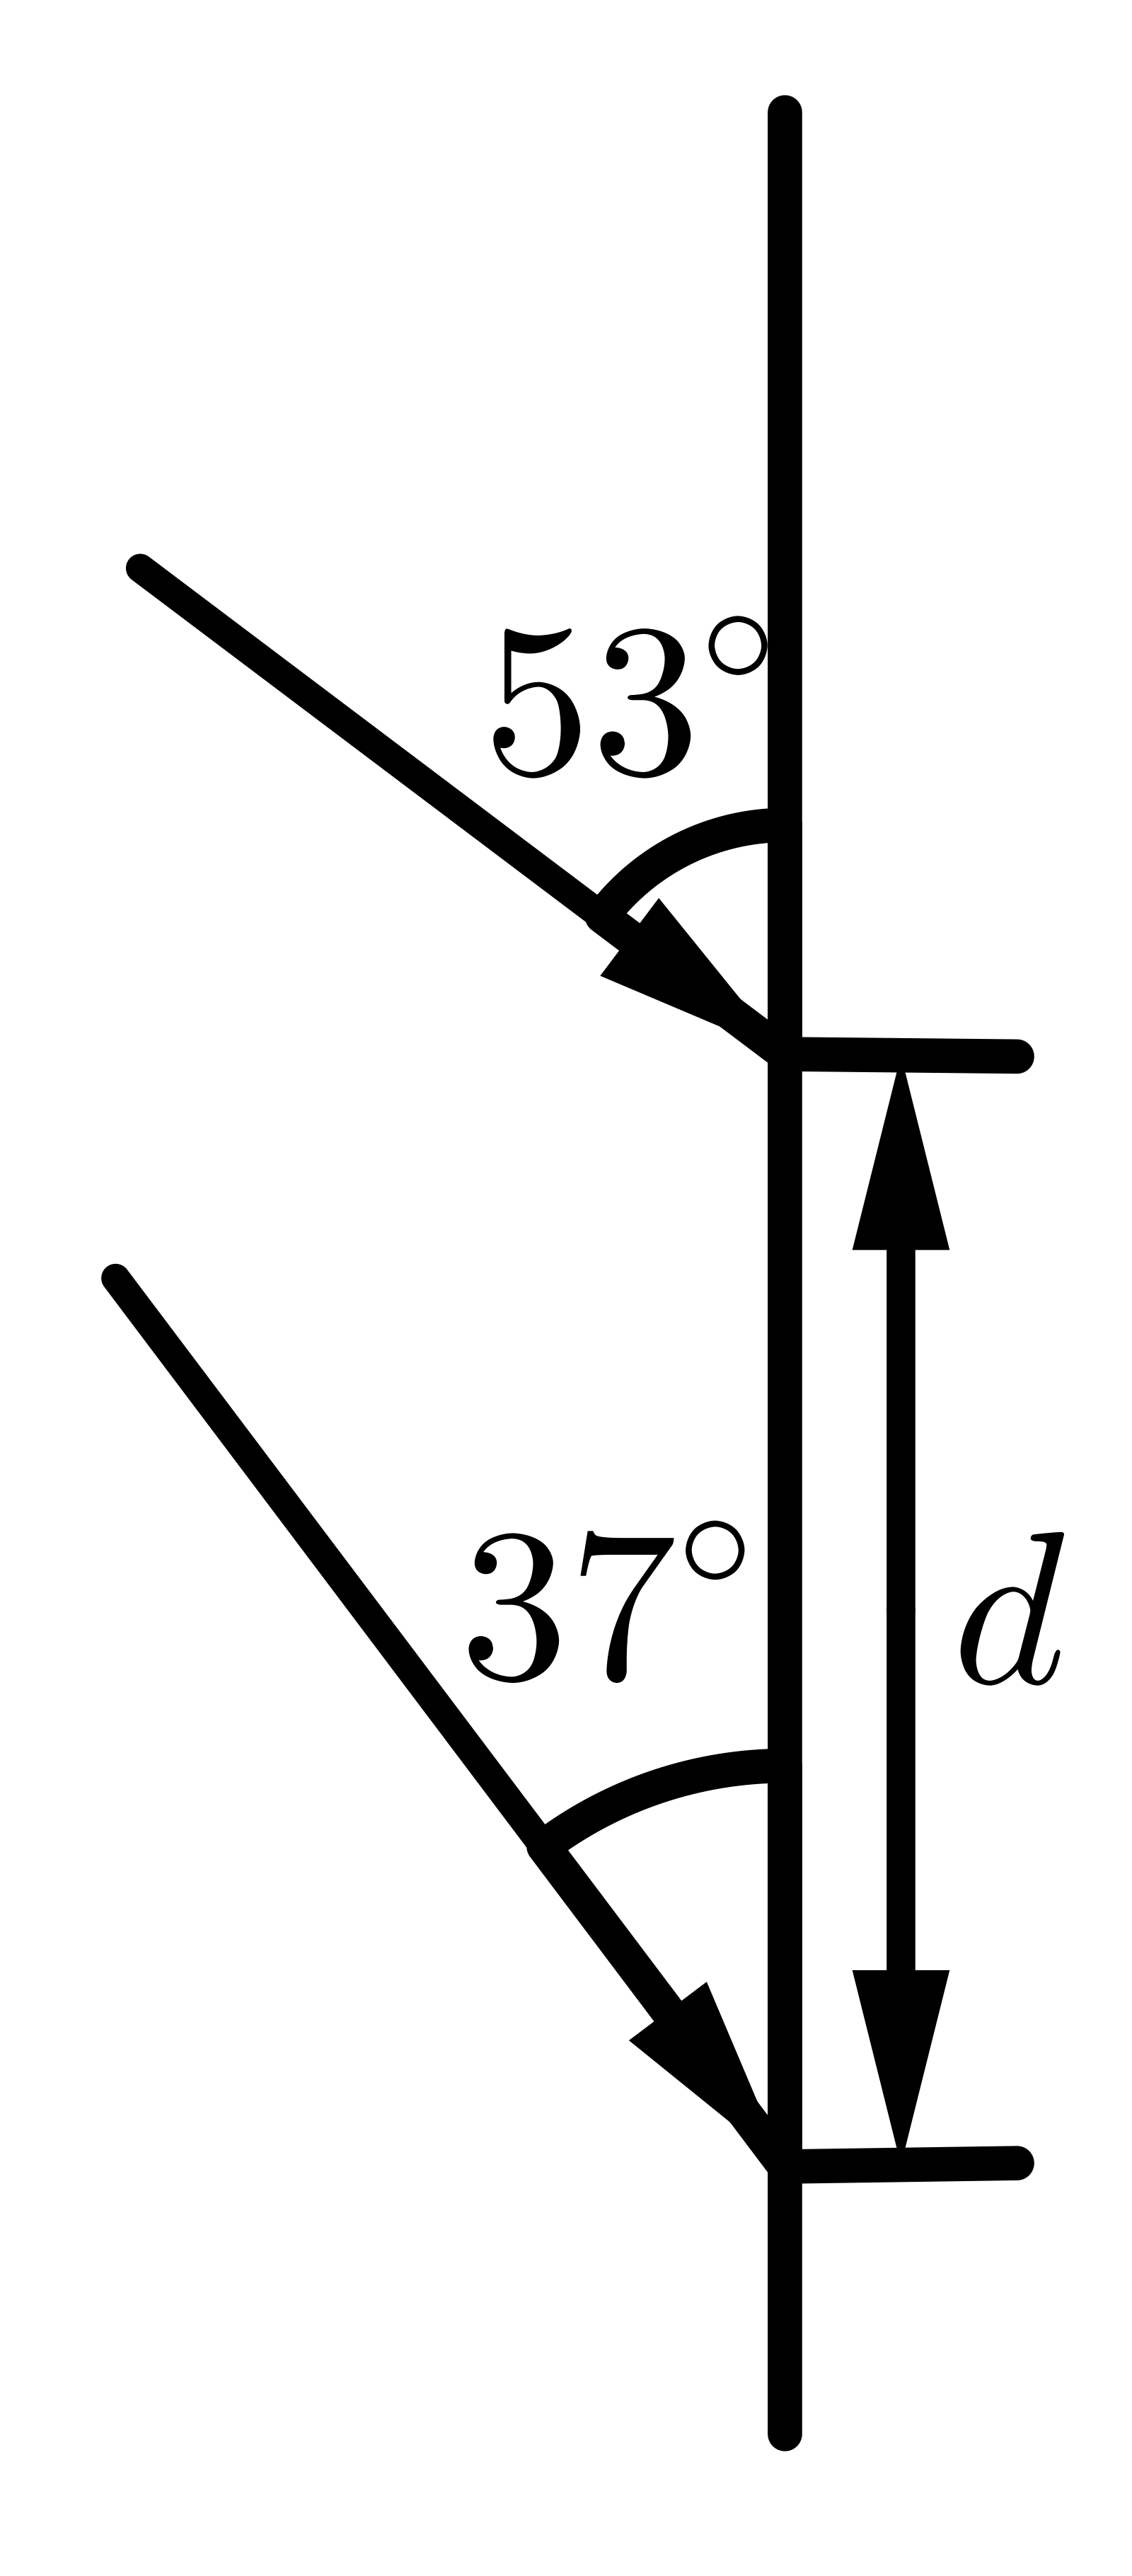
\includegraphics[width=0.12\textwidth]{pic/pic4.png}
	\label{fig4}
\end{wrapfigure}

\refstepcounter{exam}
\subparagraph{例\theexam}
竖直墙壁上落有两只飞镖,它们是从同一位置水平射出的.飞镖A在飞镖B的上方,两者间的距离为$d$.
飞镖A与竖直墙壁成$53^{\circ}$角,飞镖B与竖直墙壁成$37^{\circ}$角,假设飞镖的运动是平抛运动,
求射出点与墙壁间的水平距离.(已知$\sin 37^{\circ}=0.6,\cos 37^{\circ}=0.8$)

\textbf{解}\ \ \ 平抛运动的竖直分运动是自由落体,对于一个飞镖来说,
它的竖直位移$y$与时间$t$的关系是
\begin{equation*}
	y=\frac12gt^2.
	\tag{i}
\end{equation*}

题目中所给的距离$d$,就是两个飞镖的竖直位移差,我们需要分别求出这两个飞镖的竖直位移.
由于 (i) 式中的$t^2$是未知的,我们接下来要把它代换为已知量.

飞镖与竖直墙壁的夹角$\theta$,实际上就是末速度与竖直方向的夹角,即末速度与初速度
夹角的余角.对于一个飞镖来说,设它的初速度为$v_0$,则
\begin{equation*}
	\tan \theta=\frac{v_0}{v_y}=\frac{v_0}{gt}.
	\tag{ii}
\end{equation*}

平抛运动的水平分运动是匀速直线运动,对于一个飞镖来说,它的水平位移$x$和时间$t$的关系是
\begin{equation*}
	x=v_0t.
	\tag{iii}
\end{equation*}

(ii) 式中的$t$在分母上,(iii) 式中的$t$在分子上,将它们联立,刚好可以求出
\begin{equation*}
	t^2=\frac{x}{g\tan \theta}.
	\tag{iv}
\end{equation*}


把 (iv) 式代入 (i) 式中,得
\begin{equation*}
	y=\frac12 g\cdot \frac{x}{g\tan \theta}=\frac{x}{2\tan \theta}.
	\tag{v}
\end{equation*}

根据 (v) 式,依题意有
\begin{equation*}
	\frac{x}{2\tan 37^{\circ}}-\frac{x}{2\tan 53^{\circ}}=d,
	\tag{vi}
\end{equation*}
解得 $x=\displaystyle\frac{24}{7}d.$

因此,射出点与墙壁间的水平距离为$\displaystyle\frac{24}{7}d$.

本题的难点在于主方程的确定.由于所求量是水平位移,我们很容易误把 (iii) 式看作主方程,
然而,(iii) 式中的量均为未知量,我们无从下手.其实,主方程是把已知量与所求量建立直接联系
的式子,所以(vi) 式才是主方程.

\subsection{起落于斜面的平抛运动}

在一个斜面上以不同的速度(使物体均落于斜面)分别水平抛出两个相同物体,哪个物体先落到斜面上呢?

\begin{wrapfigure}{r}{6cm}
	\flushright
	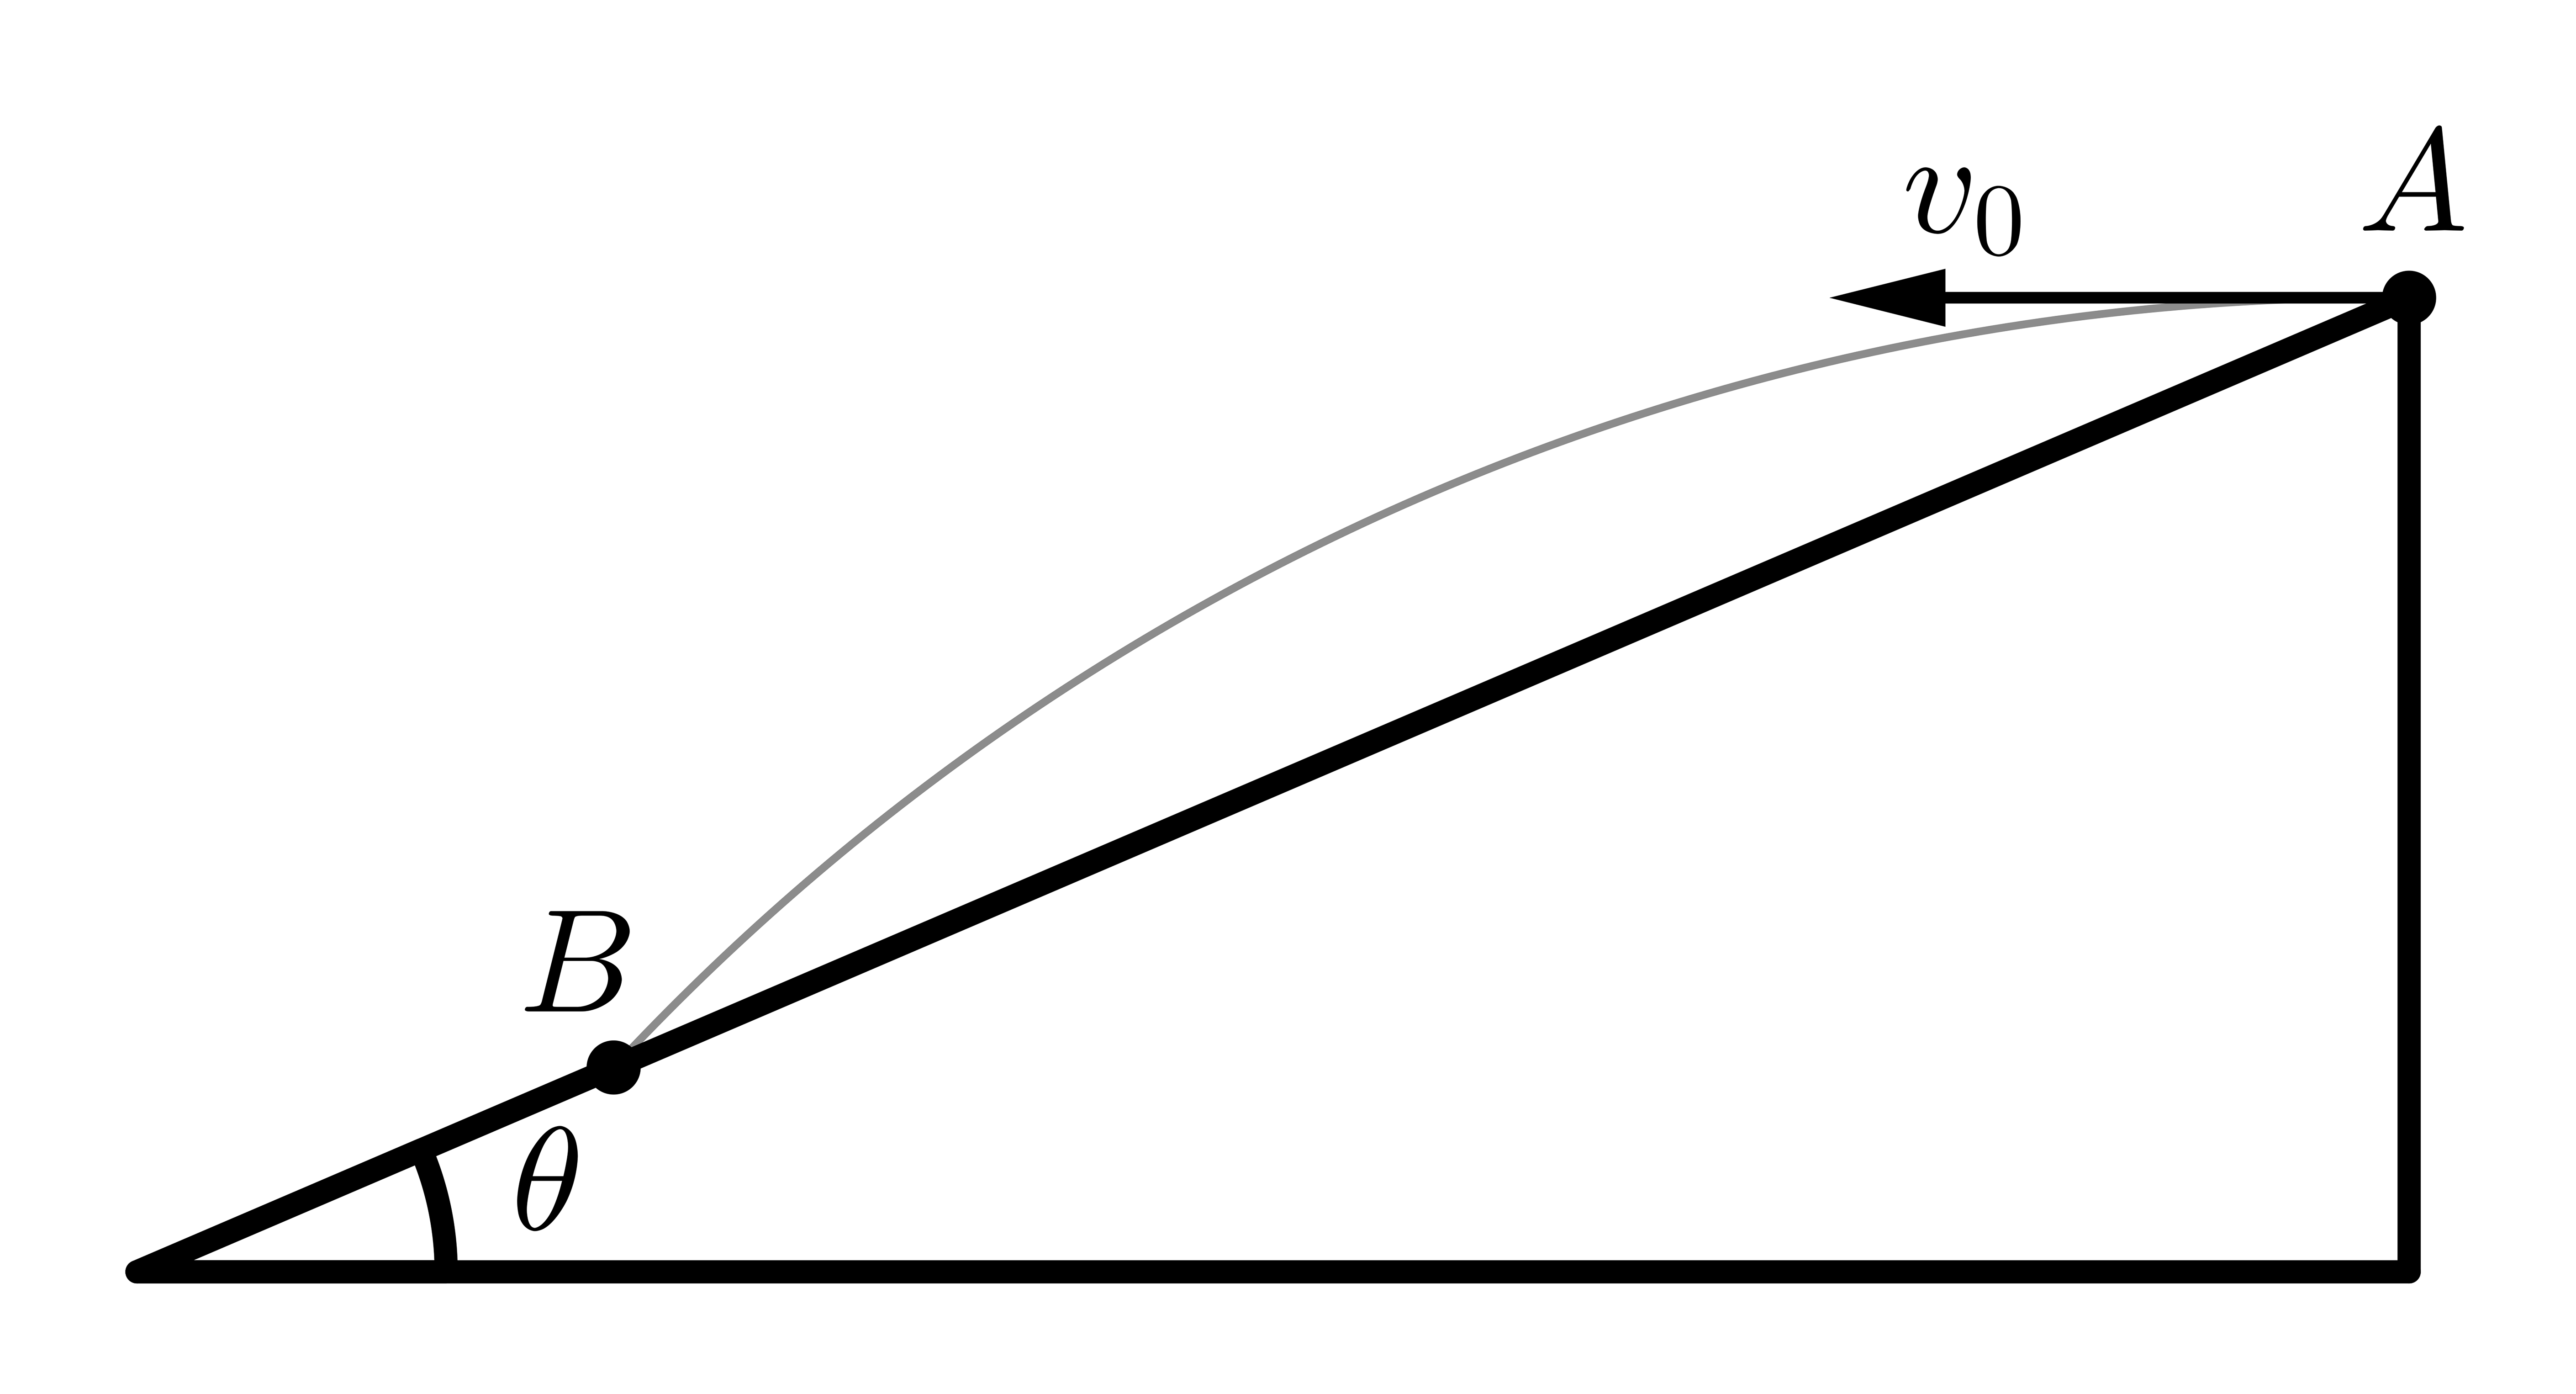
\includegraphics[width=0.4\textwidth]{pic/pic2.png}
	\label{fig2}
\end{wrapfigure}

我们先研究抛出一个物体的情况:

如图,以速度$v_0$从斜面上$A$点处水平抛出一物体,该物体做平抛运动.在保证其落于斜面
且不发生反弹的前提下, 水平分位移$x$与竖直分位移$y$的关系是
$$\frac{y}{x}=\tan{\theta}.$$
所以$$\tan{\theta}=\frac{\frac{1}{2}gt^2}{v_0t}=\frac{gt}{2v_0}.$$

于是可以解出物体在斜面上的运动时间
\begin{equation}
	t=\frac{2v_0\tan{\theta}}{g}.
	\label{斜面上的运动时间}
\end{equation}

在斜面倾角固定的情况下,上式中的$\tan{\theta}$以及重力加速度$g$都是定值,
这就是说,\textbf{物体在做起落于斜面上的平抛运动时,其运动时间与物体的初速度成正比},即
\begin{empheq}[box=\fbox]{equation}
	t\propto{v_0}.
\end{empheq}

有了运动时间,根据匀速直线运动位移$x$与时间$t$的关系,代入(\ref{斜面上的运动时间})式,
就可以得到物体在斜面上的水平位移
$$x=v_0t=v_0\cdot\frac{2v_0\tan{\theta}}{g}=\frac{2{v_0}^2\tan{\theta}}{g}.$$
再根据几何关系, 容易得到合位移
$$s=\frac{2{v_0}^2\sin{\theta}}{g\cos^2{\theta}}.$$

这就是说,\textbf{物体在做起落于斜面上的平抛运动时,其位移与物体的初速度的平方成正比},即
\begin{empheq}[box=\fbox]{equation*}
	s\propto{{v_0}^2}.
\end{empheq}

最后来研究物体的末速度.末速度的大小是容易求出的,并且有
$v\propto{v_0}$.我们重点研究末速度的方向.设物体落在斜面上时的速度$v$(水平分量$v_x$,竖直分量$v_y$)
与初速度$v_0$的夹角为$\theta_v$,则有$\tan{\theta_{v}=\displaystyle\frac{v_x}{v_y}}$.根据平抛运动的
运动规律, $v_x=v_0$, $v_y=gt$,代入(\ref{斜面上的运动时间})式,得$v_y=2v_0\tan{\theta}$,
所以
$$\tan{\theta_v}=\frac{2v_0\tan{\theta}}{v_0}=2\tan{\theta}.$$

这就表明,\textbf{物体在做起落于斜面上的平抛运动时,末速度的方向只与斜面倾角有关,与初速度无关}.
这与推论1的结论一致.

\section{圆周运动}
\subsection{圆周运动的基本概念}
\subsubsection{线速度\ \ 角速度}

在圆周运动中,把物体运动沿着一段圆弧运动的瞬时速度叫做\textbf{线速度},用符号$v$表示
$$v=\frac{\Delta{s}}{\Delta{t}}, $$
其中$\Delta s$是弧长.线速度的方向为物体做圆周运动时该点的切线方向.
应该注意的是,线速度描述的是物体在做圆周运动时某一时刻的速度,而不是平均速度.

在圆周运动中,把物体在一段时间内转过的角度$\Delta{\theta}$与所用时间$\Delta{t}$的
比值叫做\textbf{角速度},用符号 $\omega$ 表示
$$\omega=\frac{\Delta{\theta}}{\Delta{t}}.$$
在国际单位制中,角速度的单位是$\rm{rad/s}$或$s^{-1}$.

在$\Delta \theta$以弧度为单位时,因为$\Delta \theta=\displaystyle\frac{\Delta s}{r}$
(其中$s$为弧长, $r$为圆周运动的半径),所以 $$v=\omega r.$$

根据线速度与角速度的定义, 容易知道:
\begin{enumerate}
	\item \textbf{做圆周运动的物体上的各点角速度相同, 并且}$\displaystyle\frac{v_1}{v_2} = \displaystyle\frac{r_1}{r_2}.$
	\item \textbf{同轴转动的不同物体, 它们上面的各点角速度相同, 并且}$\displaystyle\frac{v_1}{v_2} = \displaystyle\frac{r_1}{r_2}.$
	\item \textbf{用皮带或齿轮传动的两个物体, 它们边缘上的点线速度相同, 并且}$\displaystyle\frac{\omega_1}{\omega_2} = \displaystyle\frac{r_2}{r_1}.$
\end{enumerate}

\subsubsection{周期}
周期是物体转过一周所用的时间,用符号$T$表示.

根据周期的定义,可知角速度$\omega$和周期$T$的关系 $$\omega=\frac{2\pi}{T};$$
线速度$v$和周期$T$的关系 $$v=\frac{2\pi r}{T}, $$其中$r$是圆周运动的半径.

\subsubsection{频率\ \ 转速}
频率是指物体在单位时间内转过的圈数,用符号$F_\mathrm{f}$表示,单位是赫兹(Hz).
频率是周期的倒数,即
$$f=\frac{1}{T}.$$

转速也是指物体在单位时间内转过的圈数,用符号$n$表示,单位是转每秒.
转速在数值上等于频率.

\subsubsection{向心力\ \ 向心加速度}
做圆周运动的物体,速度的方向时刻都在改变.牛顿第一定律告诉我们,
物体在做圆周运动时,一定受到一个外力,使它的速度总是沿着此处的切线方向,
这个力(或这个力的一个分力)指向圆心,称为\textbf{向心力},用符号$F_\mathrm{n}$表示.
物体受到指向圆心的力,是物体做圆周运动的原因.经科学技术测定,向心力的大小
$$F_\mathrm{n}=m\frac{v^2}{r}=m{\omega}^{2}r=mv\omega=m \left(\frac{2\pi}{T}\right)^2r.$$

向心力产生的加速度是\textbf{向心加速度},用符号$a_\mathrm{n}$表示.任何做匀速圆周运动的物体,其加速度都指向圆心.
向心加速度的大小描述线速度方向改变的快慢.

变速圆周运动的合加速度并不指向圆心.可以将该加速度分解,指向圆心的分量即为这个变速圆周
运动的向心加速度;沿切线方向的分量称为切向加速度,它描述线速度大小改变的快慢.
根据牛顿第二定律
$$a_\mathrm{n}=\frac{v^2}{r}={\omega}^{2}r=v\omega=\left(\frac{2\pi}{T}\right)^2r.$$

需要注意的是,向心力属于效果力,实际上就是物体所受合外力沿半径方向的分力.
如果在分析物体实际所受各力之后,又另加一个向心力,那就不对了.

\subsection{水平面上的圆周运动}

\begin{wrapfigure}{r}{5cm}
	\flushright
	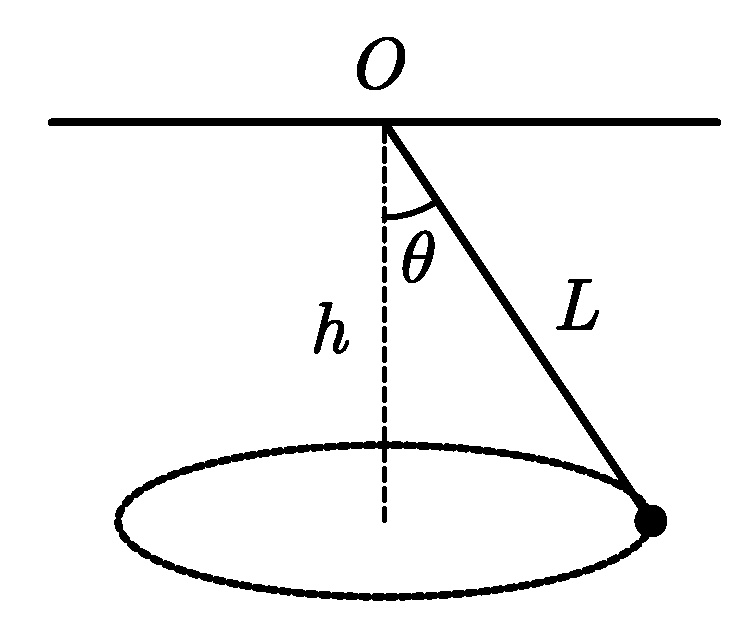
\includegraphics[width=0.3\textwidth]{pic/pic8.pdf}
	\label{fig8}
\end{wrapfigure}

我们已经知道, 向心力是一种效果力, 可以由某一性质的力提供, 也可以由某几个力的合力或某一个力的分力来提供.
分析向心力的一般步骤是:

\begin{wrapfigure}{r}{5cm}
	\flushright
	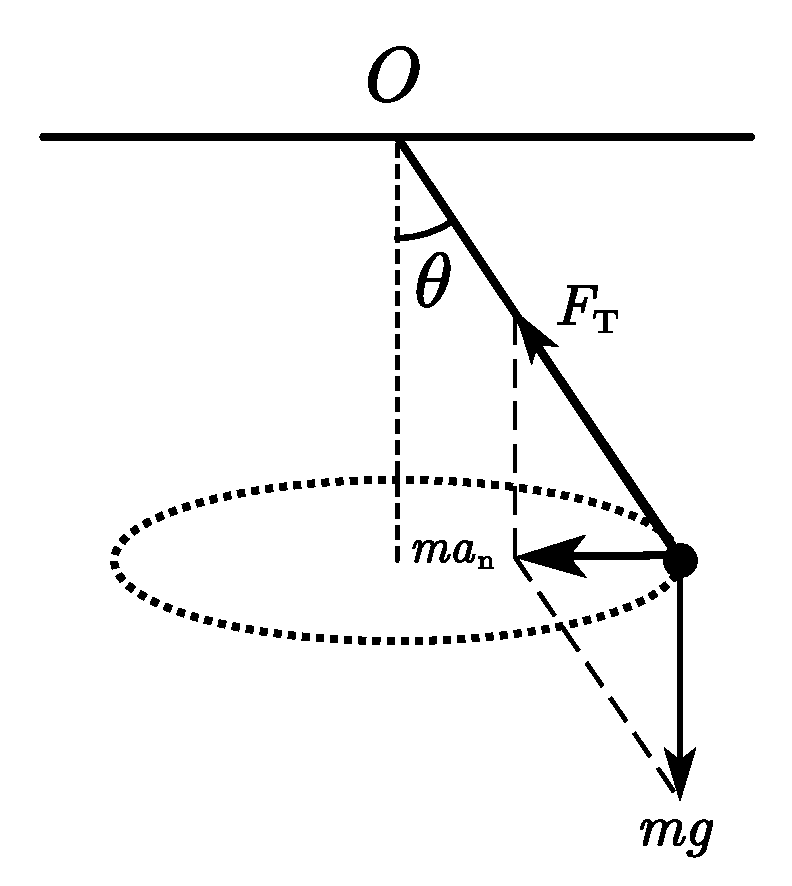
\includegraphics[width=0.3\textwidth]{pic/pic9.pdf}
	\label{fig9}
\end{wrapfigure}

(1) 确定圆周运动轨道所在的平面;

(2) 找出圆周轨道的圆心的位置;

(3) 分析做圆周运动的物体所受的力, 并作出受力图, 其中指向圆心的合力(或分力)就是向心力.

本页图中的模型叫做\textbf{圆锥摆}.我们以它为例进行分析.

如右图, 长为$L$的细线上栓一质量为$m$的小球, 细线一端固定于$O$点, 让其在水平面内做匀速圆周运动.
这种运动一般称为圆锥摆运动, $h$称为摆高. 细线与竖直方向的夹角为$\theta$.

在找出圆周轨道所在平面以及圆心之后, 我们对小球进行受力分析, 如右图. 因为小球做匀速圆周运动, 所以
小球受到的向心力大小是恒定的. 由受力分析可知, 小球的做圆周运动的向心力就是它受到的拉力与重力的合力,
并且有
\begin{equation}
	F_\mathrm{T} \cos \theta = mg,
	\label{圆锥摆1}
\end{equation}
\begin{equation}
	mg \tan \theta = ma_\mathrm{n}.
	\label{圆锥摆2}
\end{equation}

由(\ref{圆锥摆1})解得$F_\mathrm{T} = \displaystyle\frac{mg}{\cos \theta}$,
由(\ref{圆锥摆2})解得
\begin{equation}
	a_\mathrm{n} = g\tan \theta.
	\label{圆锥摆3}
\end{equation}

由于$a_\mathrm{n}=\omega^2 r$, 又由几何关系得$r = h \tan \theta$, 结合(\ref{圆锥摆3})
有$$g\tan \theta = \omega^2 h \tan \theta.$$
由此解得, 小球做圆锥摆运动的角速度$$\omega = \sqrt{\frac{g}{h}}.$$
这就是说, \textbf{在圆锥摆运动中, 物体的角速度的平方与摆高成反比},即$$\omega^2 \propto \frac{1}{h}.$$

同理, 由$a_\mathrm{n}=(\displaystyle\frac{2\pi}{T})^2r$, $r = L \sin \theta$, 以及(\ref{圆锥摆3}), 得
$$g\tan \theta = \left(\displaystyle\frac{2\pi}{T}\right)^2 L \sin \theta.$$
由此解得, 小球做圆锥摆运动的周期$$T = 2\pi \sqrt{\frac{L \cos \theta}{g}}.$$

\subsection{竖直平面上的圆周运动}

\subsubsection{竖直圆周的动力学分析}

用轻绳拉着小球在竖直面内做圆周运动,将小球所受的重力分解为沿半径
方向的$G_1$和沿切线方向的,垂直于$G_1$的$G_2$.

$G_1$提供小球的(一部分或全部)向心力,改变速度的方向.
当绳提供的力不为0时, 小球的向心力是$G_1$与拉力的合力.

$G_2$提供小球的切向力, 改变速度的大小.特别地, 当小球在最高点和最低点时, $G_2 = 0$, 即小球的切向力为0.
因此小球的速率不变. 一般时刻, 在竖直面做圆周运动的小球做\textbf{变速圆周运动}.

当小球在圆周的下半部分时, 绳子的拉力$F$与$G_1$反向. 所以有
$F - G_1 = m\displaystyle\frac{v^2}{r}.$即$$F = mg\cos \theta + m\frac{v^2}{r}.$$
其中$\theta$为绳与竖直方向的夹角.
小球位置越高, $\theta$越大, 小球运动的线速度$v$越小, 绳子的拉力$F$越小.
并且$F$在最低点处取得最大值$$F_\mathrm{max} = m\frac{v^2}{r} + mg.$$

同理, 小球在圆心上方时, 绳子的拉力 $$F = mg\cos \theta - m\frac{v^2}{r}.$$
小球位置越高, $\theta$越小, 小球运动的线速度$v$越小, 绳子的拉力$F$越小.
并且$F$在最高点处取得最小值
\begin{equation}
	F_\text{min} = m\frac{v^2}{r} - mg.
	\label{最小拉力}
\end{equation}
当然, 前提是小球能上升到最高点, 并且能持续圆周运动. 这就需要小球在到达最高点时
有速度, 并且绳子拉直.

下面我们来研究小球能到达最高点的条件.

\subsubsection{竖直圆周的临界问题}

通过受力分析可知, 物体在竖直平面内做圆周运动时,一般在通过最高点时处于临界状态.下面我们来
研究一下这个问题.

我们知道, 当$F_\text{min} = 0$时, 小球恰好能到达最高点.由(\ref{最小拉力})可知
临界条件是$mg = m\displaystyle\frac{v_0^2}{r}$ (式中$v_0$是小球恰达最高点时的速度).由此解得
\begin{equation}
	v_0 = \sqrt{gr}.
	\label{临界速度}
\end{equation}

这就是说, \textbf{在竖直平面内被绳子牵引做圆周运动的物体, 能通过最高点并继续运动的条件是, 小球通过最高点时
	的速度$v \geqslant \sqrt{gr}.$}

当小球在最高点处的速度小于这个值时, 那么$mg \textgreater m\displaystyle\frac{v^2}{r}, $小球将靠近圆周轨道, 称为\textbf{近心运动}.

如果小球用杆牵引,或在管径略大于小球直径的管道内运动, 那么只需过最高点时的的速度大于0, 小球即可完成圆周运动.
如果小球到达最高点时, 与支撑物(杆或管道)间无相互作用, 那么小球在这一点的速度$v = \sqrt{gr}$.

学习动能定理后, 解决此类问题将变得容易许多.
\subsection{生活中的圆周运动}

\subsubsection{汽车过拱桥\ \ \ 汽车过地道}

汽车通过拱桥时, 实际是在做竖直面上的圆周运动. 当汽车在拱桥的最高点时, 汽车所受的重力大于支持力, 发生失重现象.
视拱桥为圆弧, 其半径为$r$.
设汽车的质量为$m$, 汽车所受的支持力为$F_\mathrm{N}$, 汽车在最高点时的速度为$v$, 重力加速度为$g$.
对汽车进行受力分析, 可得$$mg - F_\mathrm{N} = m\frac{v^2}{r}.$$
由此可知, 随着汽车速度$v$的增大, 汽车所受的支持力$F_\mathrm{N}$减小. 当支持力减小到0时, 汽车做平抛运动,
此时$$mg = m\frac{v^2}{r},$$ 解得$v = \sqrt{gr}.$

汽车通过地道时, 所受的重力小于支持力, 发生失重现象. 使地道为圆弧, 其半径为$r$.
设汽车的质量为$m$, 汽车所受的支持力为$F_\mathrm{N}$, 汽车在最高点时的速度为$v$, 重力加速度为$g$.
对汽车进行受力分析, 可得$$F_\mathrm{N} - mg = m\frac{v^2}{r}.$$
由此可知, 随着汽车速度$v$的增大, 汽车所受的支持力$F_\mathrm{N}$也随之增大. 如果汽车速度过快, 可能会爆胎.

\subsubsection{汽车拐弯}

\begin{wrapfigure}{r}{5cm}
	\flushright
	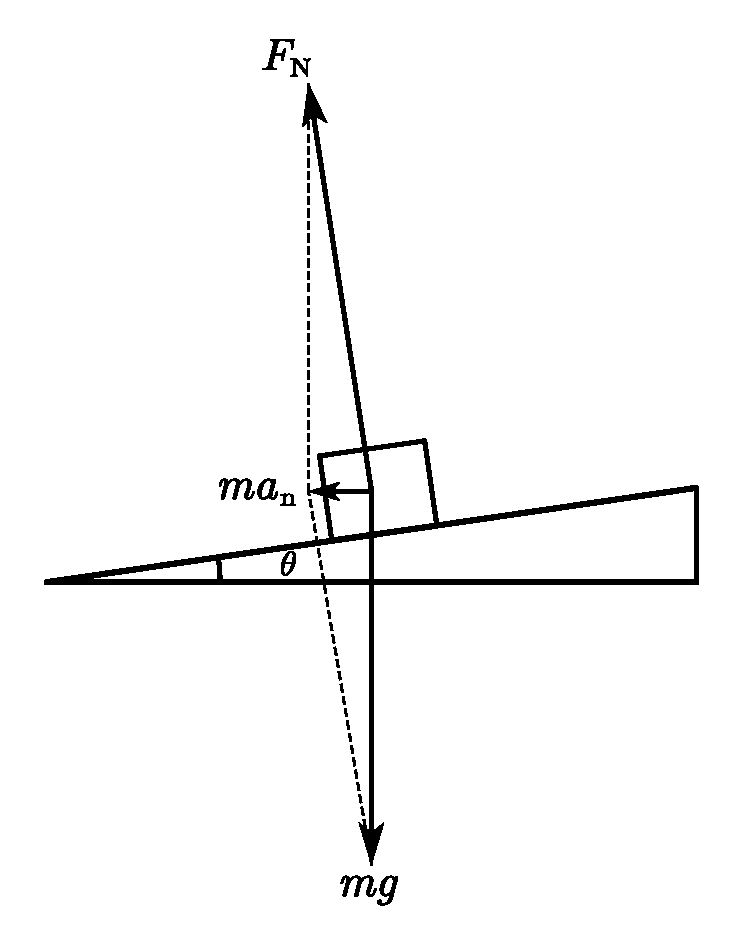
\includegraphics[width=0.3\textwidth]{pic/pic12.pdf}
	\label{fig12}
\end{wrapfigure}


汽车拐弯时, 实际是在做水平面上的圆周运动. 视弯道为一段圆弧, 其半径为$r$. 汽车拐弯的向心力由静摩擦力$F_\mathrm{f}$
提供$$F_\mathrm{f} = m\frac{v^2}{r}.$$因为$F_\mathrm{f}$有最大值, 所以当速度$v$过大时, 静摩擦力$F_\mathrm{f}$
可能无法提供向心力.

当$F_\mathrm{f} \textless m\displaystyle\frac{v^2}{r}$时, 摩擦力小于汽车所需的向心力,
汽车将会远离原圆周运动的轨道,称为\textbf{离心运动}.这是很危险的.

为了防止发生危险, 弯道一般会做成倾斜的, 火车轨道更会严格的设计倾斜角度, 这是为了让$mg$与$F_\mathrm{N}$产生
水平合力, 从而提供拐弯所需的向心力$$m\frac{v^2}{r} = mg\tan \theta.$$
由此可得, 当$v = \sqrt{gr\tan \theta}$时, 汽车与地面间无摩擦力.

在这样的设计下, 即使汽车的速度略超过临界速度$\sqrt{gr\tan \theta}$, 也不易发生危险, 因为静摩擦力会补上所需的那部分力.

飞机在转弯时倾斜机身, 也是因为这一点.

\section{万有引力与宇宙航行}

\subsection{万有引力}

\subsubsection{行星运动的科学史}

在古代,人们对于天体运动存在着地心说和日心说两种对立的看法. 地心说是托勒密提出的, 日心说是哥白尼提出的. 最终,
日心说战胜了地心说, 被人们所接受.

德国天文学家开普勒后续发现, 行星绕太阳运动的轨道不是圆, 而是椭圆, 并
于1609年和1619年, 发表了他发现的下列规律, 后人称为开普勒行星运动定律.

\subparagraph{开普勒第一定律}所有行星绕太阳运动的轨道都是椭圆,太阳处在椭圆的一个焦点上.

\subparagraph{开普勒第二定律} 对任意一个行星来说,它与太阳的连线在相等的时间内扫过的面积相等.

开普勒第二定律告诉我们:当行星离太阳较近的时候,运行的速度较大,而离太阳较远的时候速度较小.

\subparagraph{开普勒第三定律} 所有行星轨道的半长轴的三次方跟它的公转周期的二次方的比都相等.

若用 $a$ 代表椭圆轨道的半长轴, $T$代表公转周期,开普
勒第三定律告诉我们$$\frac{a^3}{T^2} = k, $$其中比值$k$是一个对所有行星都相同的常量.
事实上, \textbf{它由太阳的质量决定}.

实际上, 行星的轨道与圆十分接近.在中学阶段,我们仍按圆轨道处理,这样就可以说:
\begin{enumerate}
	\setlength{\itemsep}{0pt}
	\setlength{\parsep}{0pt}
	\setlength{\parskip}{0pt}
	\item 行星绕太阳运动的轨道十分接近圆,太阳处在圆心.
	\item 对某一行星来说,它绕太阳做圆周运动的角速度
	      (或线速度)大小不变,即行星做匀速圆周运动.
	\item 所有行星轨道半径 $r$ 的三次方跟它的公转周期 $T$ 的二
	      次方的比值都相等, 即$\displaystyle\frac{r^3}{T^2} = k.$
\end{enumerate}

\subsubsection{万有引力}

根据开普勒第三定律, 圆周运动加速度表达式, 可以推出行星与太阳间的作用力$$F = G \frac{m_\text{太}m}{r^2}, $$
其中$G$是常数, $m$是行星的质量, $m_\text{太}$是太阳的质量.太阳与行星间引力的方向沿着二者的连线.

``月地检验''告诉我们, 地面上的物体所受地球的引力,月球所受地球的引力,以及太阳与行星间的引力,都遵从相同的规律.

事实上, 任意两个物体间都有引力, 只是因为它们的质量相比于天体很小, 难以发现罢了.于是我们有
\subparagraph{万有引力定律} 自然界中任何两个物体都互相吸引,引力的方向在他们的连线上,引力的大小
与物体的质量$m_1$, $m_2$的乘积成正比,与它们之间距离$r$的二次方成反比,即
\begin{empheq}[box=\fbox]{equation*}
	F = G\ \frac{m_1 m_2}{r^2},
\end{empheq}
其中质量的单位用千克,距离的单位用米,力的单位用牛.$G$是比例系数,叫做引力常量,适用于任何两个物体, $$G \approx 6.67 \times 10^{-11}\ \mathrm{N\cdot m^2 \cdot kg^{-2}}.$$

\subsubsection{称量天体的质量}

\textbf{方法 1}\ \ \ 已知引力常数$G$, 和某绕转天体的任意两个运动参量(线速度,角速度,加速度,绕转半径), 由万有引力等于向心力,
可以解出中心天体的质量.

\textbf{方法 2}\ \ \ 已知引力常数$G$和天体的半径$R$, 再测定出该天体表面的的重力加速度$g$, 由$mg = G\displaystyle\frac{Mm}{R^2}$, 可以解出天体的质量$M$.

\subsection{万有引力与重力}

\setlength{\abovedisplayskip}{3pt}
\setlength{\belowdisplayskip}{3pt}

物体与地球间的万有引力实际上就是物体随地球转动的向心力与物体受到的重力重力的合力.因此,
不计地球自转时,重力就是物体与地球间的万有引力.

\subparagraph{1. 地球表面的重力加速度}地球表面一质量为$m$的物体,在不考虑地球自转的情况下,它的重力就是它与地球间的万有引力.
已知地球的质量为$M$,地球半径(视地球为正球体)为$R$,万有引力常数为$G$,则有
$$mg=G\frac{Mm}{R^2}.$$

即
\begin{empheq}[box=\fbox]{equation}
	g=G\frac{M}{R^2}.
	\label{重力加速度}
\end{empheq}
这是\textbf{不计地球自转时, 地球上一点的重力加速度的决定式}.

\subparagraph{2. 不同高度处的重力加速度}

物体在距地表 $h$处的空中, 那么 (\ref{重力加速度}) 中$R$替换为${R+h}$,即
$$g'=G\frac{M}{(R+h)^2}.$$

\subparagraph{3. 不同深度处的重力加速度}

物体在地下深度为 $H$ 处, 因为物体上方的``球壳''对物体没有引力, 所以
\begin{align*}
	g' & =G\frac{(\frac{R-H}{R})^3M}{(R-H)^2} \\
	   & =\frac{GM(R-H)}{R^3}                 \\
	   & =\frac{GM}{R^2}\cdot\frac{R-H}{R}    \\
	   & =g\ \frac{R-H}{R}.
\end{align*}
其中$g$是地球表面的重力加速度.

于是就有
$$\frac{g'}{g}=\frac{R-H}{R}.$$

如果考虑地球自转,那么物体在地球上受到的重力就等于物体与地球间的万有引力与物体随地球做圆周运动
(一般视为匀速圆周运动)的向心力的差.特别地,当物体在极点上时,不会随地球自转而运动,即仍有
$$mg=G\frac{Mm}{R^2}.$$

当物体在赤道上时,物体做圆周运动的半径就是地球半径,并且向心力与引力同向
$$mg=G\frac{Mm}{R^2}-m\omega^2R.$$

一般地,当物体在地球上某一点时,它们之间的万有引力就是物体受到的重力与向心力的矢量和.

\subparagraph{黄金代换式}

由(\ref{重力加速度})可得
\begin{empheq}[box=\fbox]{equation}
	GM = gr^2.
	\label{黄金代换式}
\end{empheq}
式中$G$是引力常数, $M$是地球质量, $r$是地球中心与物体的距离, $g$是物体在距地球中心$r$处的重力加速度.

这个式子常用于$GM$与$gr^2$之间的代换, 称为黄金代换式.

\subsection{万有引力与宇宙航行}

本节我们研究卫星绕地球运动的问题.
由于卫星与地球的距离较远, 根据 \eqref{重力加速度} 可知, 卫星所受的重力非常小,
所以我们只研究万有引力与圆周运动的向心力之间的关系.

\subsubsection{宇宙航行的定量计算}

因为卫星绕地球运动的向心力由卫星与地球间的万有引力提供, 设地球质量为$M$, 卫星质量为$m$,
卫星中心与地球中心的距离为$r$, 卫星的线速度为$v$, 角速度为$\omega$, 向心加速度为$a_\mathrm{n}$,
万有引力常数为$G$, 有
\begin{equation}
	G\frac{Mm}{r^2} = m\frac{v^2}{r},
	\label{宇宙航行1}
\end{equation}
\begin{equation}
	G\frac{Mm}{r^2} = m\omega^2 r,
	\label{宇宙航行2}
\end{equation}
\begin{equation}
	G\frac{Mm}{r^2} = ma_\mathrm{n}.
	\label{宇宙航行3}
\end{equation}

由 \eqref{宇宙航行1} 可得$v = \sqrt{\displaystyle\frac{GM}{r}}$, 即$v\propto \sqrt{\displaystyle\frac1r}$.\par\vspace{8pt}
由 \eqref{宇宙航行2} 可得$\omega = \sqrt{\displaystyle\frac{GM}{r^3}}$, 即$\omega \propto \sqrt{\displaystyle\frac{1}{r^3}}$.\par\vspace{8pt}
由 \eqref{宇宙航行3} 可得$a_\mathrm{n} = \displaystyle\frac{GM}{r^2}$, 即$a_\mathrm{n}\propto \displaystyle\frac{1}{r^2}$.

\subsubsection{宇宙航行的定性分析}

由前面的分析, 我们可以知道, 当卫星的绕转半径$r$一定时, 它的线速度, 角速度, 向心加速度以及周期都是一定的, 这保证了
卫星间的相对位置稳定, 不会相撞.

当卫星的绕转半径$r$增大时, 根据前面的分析, 卫星的线速度$v$减小; 向心加速度$a_\mathrm{n}$减小; 角速度$\omega$减小,
由$\omega = \displaystyle\frac{2\pi}{t}$知周期$T$增大. 这就是\textbf{``高轨低速大周期''}.

我们把卫星的线速度, 角速度(周期), 向心加速度, 绕转半径称为卫星的运动参量, 知道它们中的两个, 就可以求出另外两个.
当卫星的质量未知时, 引力值是无法求出的.

\subsubsection{三种宇宙速度}

\subparagraph{第一宇宙速度} 使卫星能环绕地球运行所需的最小发射速度叫做第一宇宙速度.
当卫星以第一宇宙速度$v_1$发射时, 它将绕地球做匀速圆周运动. 设地球质量为$M$, 卫星的
质量为$m$, 它到地心的距离为$r$. 由于卫星做圆周运动所需的向心力由万有引力提供, 因此
有$$G\frac{Mm}{r^2} = m\frac{v^2}{r},$$解得
\begin{equation}
	v = \sqrt{\frac{GM}{r}}.
	\label{卫星绕转速度}
\end{equation}
此时$r$约等于地球半径$R$,即$v_1 = \displaystyle\sqrt{\frac{GM}{R}}$.
代入数据可解得$$v_1 \approx 7.9\ \mathrm{km/s}.$$

除此之外, 根据黄金代换式 \ref{黄金代换式} 和(\ref{卫星绕转速度}),我们可以得到卫星绕转速度的另一种表达式$$v = \sqrt{gr},$$
但这并不能说明卫星的绕转速度与$\sqrt{r}$成正比,因为在卫星的高度增加时, $g$的值也在变化,
并且$g = \displaystyle\frac{GM}{r^2}$.

事实上, 根据(\ref{卫星绕转速度}), \textbf{卫星的绕转速度$v$与$\sqrt{r}$是成反比的}.

\subparagraph{第二宇宙速度} 在地面附近发射人造卫星, 如果发射速度
$v \in (7.9\ \mathrm{km/s}, 11.2\ \mathrm{km/s})$, 那么它绕地球运行的轨迹将是椭圆.
当发射速度大于等于$11.2\ \mathrm{km/s}$时, 卫星会克服地球的引力而永远离开地球.
我们把它叫做第二宇宙速度.$$v_2 \approx 11.2\ \mathrm{km/s}.$$

\subparagraph{第三宇宙速度} 达到第二宇宙速度的人造卫星还受到太阳的引力. 在地面附近发射一颗人造卫星,
要使它摆脱太阳引力的束缚, 飞到太阳系外, 必须使其发射速度大于等于$16.7\ \mathrm{km/s}$, 这个速度叫做
第三宇宙速度.$$v_3 \approx 16.7\ \mathrm{km/s}.$$
\begin{wrapfigure}{r}{5cm}
	\flushright
	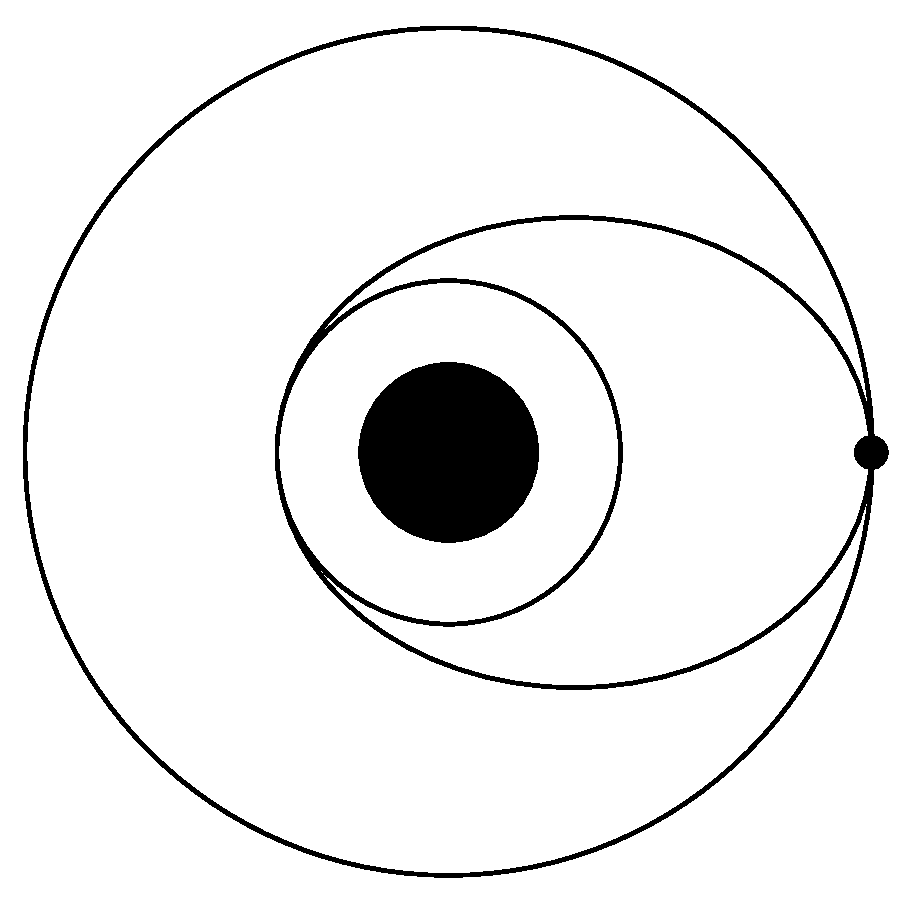
\includegraphics[width=0.28\textwidth]{pic/pic13.pdf}
	\label{fic13}
\end{wrapfigure}

\subsubsection{变轨问题}

卫星绕中心天体做匀速圆周运动时, 万有引力提供向心力. 当卫星由于某种原因速度突然改变时, 由
(\ref{宇宙航行1})可知, 万有引力不再等于
向心力, 卫星将变轨运行. 卫星的发射和回收就是利用了这一原理.

一个质量为$m$的卫星以第一宇宙速度发射, 它绕地球做匀速圆周运动. 这时, 如果该卫星喷气加速, 那么万有引力不足以
提供向心力, 卫星将做离心运动, 卫星的轨迹是一个椭圆.可以知道, 卫星在椭圆近地点的速度, 大于卫星在原匀速圆周轨道上的速度.
当卫星运行到椭圆的远地点时, 根据 \ref{卫星绕转速度}, 卫星速度减小.

如果卫星在原地点时再次加速, 调整为合适的速度, 那么卫星就可以在更大的圆周轨道上运动. 可以知道, 卫星在大圆周轨道
上的速度, 大于卫星在原椭圆轨道远地点的速度. 另外, 由于大圆周轨道与原小圆周轨道都是圆周轨道, 根据``高轨低速大周期'',
可知卫星在小圆周轨道上的速度大于卫星在大圆周轨道上的速度.

综上所述, 可以得到
$$v_\text{椭圆近地点} \textgreater v_\text{小圆周轨道} \textgreater v_\text{大圆周轨道} \textgreater v_\text{椭圆远地点}.$$

\subsubsection{双星系统}

在天体运动中,将两颗彼此距离较近的恒星称为双星.它们在相互之间的万有引力作用下,绕两
者连线上的某定点做周期相同的匀速圆周运动.双星系统具有以下三个特点:
\begin{enumerate}
	\setlength{\itemsep}{0pt}
	\setlength{\parsep}{0pt}
	\setlength{\parskip}{0pt}
	\item 两星球做圆周运动所需的向心力由两者间的万有引力提供, 因此两星球做圆周运动的向心
	      力大小相等;
	\item 两星球绕转动中心做圆周运动的角速度(或周期)的大小相等;\label{周期相等}
	\item 质量为$m_1$, $m_2$的两星球绕共同中心转动的半径$r_1$, $r_2$的和等于两星球间的距离$L$,
	      即$$r_1 + r_2 = L,$$ 并且\textbf{两星球绕转半径之比等于它们质量的反比}, 即
	      $$\frac{r_1}{r_2} = \frac{m_2}{m_1}.$$ \label{半径与距离}
\end{enumerate}

以上三个特点是解决很多双星问题(求解运动周期、角速度、轨道半径等) 的关键.

由特点\ref{周期相等}, 我们来推导双星系统运动的周期.

设这两个恒星的的质量分别为$m_1$, $m_2$, 绕转半径分别为$r_1$, $r_2$, 它们间的距离为$L$, 根据特点\ref{半径与距离},
有$r_1 + r_2 = L$.

对于$m_1$,有$$\frac{Gm_2}{L^2} = \left(\frac{2\pi}{T}\right)^2r_1, $$

对于$m_2$, 有$$\frac{Gm_1}{L^2} = \left(\frac{2\pi}{T}\right)^2r_2, $$

把上面两式相加, 得$$\frac{G(m_1 + m_2)}{L^2} = \left(\frac{2\pi}{T}\right)^2L, $$

由此可得\subparagraph{双星系统的运动周期}$$T = 2\pi \sqrt{\frac{r^3}{G(m_1 + m_2)}}.$$

\section{功和能}

\subsection{功}

\subsubsection{功的基本概念}
物体受到力的作用, 并且在力的方向上发生一段位移,我们就说,\textbf{力对物体做了功},
功的大小等于力的大小,位移的大小,力与位移夹角的余弦值三者的乘积, 即力与位移的数量积.功用$W$表示,即
\begin{empheq}[box=\fbox]{equation}
	W = Fl \cos \theta.
	\label{功的定义式}
\end{empheq}
式中$F$是物体所受的恒力, $l$是物体的受力点对地的位移.单位是焦耳(J).
$$1 \ \mathrm{J} = 1\ \mathrm{N}\cdot 1\ \mathrm{m}.$$

功是标量,只有大小没有方向.当一个物体在几个力的作用下发生一段位移时, 这几个力
对物体所做的总功, 等于各个力分别对物体所做的功的代数和.即
$W = F_{\text{合}}l\cos \theta, $或者$W = \displaystyle\sum^{n}_{i = 1}W_i.$

\subsubsection*{功的正负}

物体受一个力的作用,如果这个力使物体的能量增多了,我们就说这个力对物体做了正功;如果这个力使物体的能量减少了,
我们就说这个力对物体做了负功.

从公式$W = Fl \cos \theta$的角度来说, 因为$F$和$l$都是正数, 所以功$W$的正负由力与位移的夹角$\theta$决定.

\begin{enumerate}
	\item 当$\theta < \displaystyle\frac{\pi}{2}$ 时, $\cos \theta > 0$, $W > 0$.这说明力做正功,充当动力;

	\item 当$\theta = \displaystyle\frac{\pi}{2}$ 时, $\cos \theta = 0$, $W = 0$.这说明力不做功;

	\item 当$\theta > \displaystyle\frac{\pi}{2}$ 时, $\cos \theta < 0$, $W < 0$.这说明力做负功,充当阻力.
\end{enumerate}

某力对物体做负功,往往也说成``物体克服某力做功''.

特别地, 重力等部分主动力做功, 一般与物体实际的运动轨迹无关, 而只与物体的初末位置有关.比如重力做的功
\begin{equation*}
	W_\mathrm{G} =\pm mg\Delta h,
\end{equation*}
这样的力称为\textbf{保守力}.

\subsubsection{特殊力做功的特点}
\subsubsection*{变力做功}

前面介绍的, 功的定义式(\ref{功的定义式})仅适用于计算恒力做功, 若是变力,此公式不再适用.
在求解变力做功时,我们可以用微元法, 平均值法, 图像法, 或把变力化为恒力.当变力的功率一定时,
我们可以用$W = Pt$计算功.

\subsubsection*{一对作用力与反作用力做功\ \ \ 一对平衡力做功}

一对作用力与反作用力总是大小相等,方向相反, 但他们分别作用在两个物体上, 二者两个物体各自发生的位移是不确定的.
所以一个力做功时, 其反作用力可能做功, 也可能不做功; 可能做正功, 也可能做负功, 它们之间没有必要的联系.

一对平衡力总是大小相等, 方向相反, 作用在同一个物体上. 若物体静止, 则两个力都不做功; 若物体运动, 则这一对力
所做的功一定互为相反数.

\subsubsection*{摩擦力做功}

一个物块沿着粗糙的斜面上滑, 位移为$s$, 那么当滑到该点时, 摩擦力$F_\mathrm{f}$所做的功$$W_\mathrm{f} = -F_\mathrm{f}s.$$
若物块又从该点下滑回原点, 那么摩擦力又做功$-F_\mathrm{f}s$, 从而全程摩擦力做功为$$W_\mathrm{f} = -2F_\mathrm{f}s.$$

虽然全程的位移为0, 但由于摩擦力的方向改变了, 所以我们不能简单的用摩擦力的大小乘以位移0而得出摩擦力做功为0.

需要注意的是, 摩擦力并不总是做负功. 例如物块放在传送带上由静止开始运动时, 摩擦力就做了正功.

\subsection{功率}

我们把力对物体所做的功$W$与完成这些功所用的时间$t$之比叫做这个力的\textbf{功率}, 用$P$表示, 即
\begin{empheq}[box=\fbox]{equation}
	P = \frac{W}{t}.
	\label{功率的定义式}
\end{empheq}
功率是反应物体做功快慢的物理量, 单位是瓦特(W).

功率是标量, 只有大小没有方向. 并且一般没有负值, 也就是说 \eqref{功率的定义式} 中的$W$
实际上是$|W|$.

上述功率的定义式(\ref{功率的定义式})一般用于求平均功率. 特别地, 因为
$P = \displaystyle\frac{W}{t} = \displaystyle\frac{Fl \cos \theta}{t}$,
而当$t\rightarrow 0$时,
瞬时速度$v = \displaystyle\frac{l}{t}$, 所以
\begin{empheq}[box=\fbox]{equation}
	P = Fv \cos \theta.
	\label{瞬时功率}
\end{empheq}
\textbf{这是力$F$做功某一时刻瞬时功率的决定式}, 其中$v$是物体在这一时刻的瞬时速度, $\theta$是这一时刻
$F$与$v$的夹角.

当$v$为平均速度时, 上式也可以计算对应时间$t$内的平均功率.

从(\ref{瞬时功率})可以看出, 汽车, 火车等交通工具,当发动机的输出功率一定时, 牵引力$F$与
速度$v$成反比, 要增大牵引力, 就要减小速度.

\subsection{能量}

初中时我们知道, 功是能量转化的量度. 能量是表示物体做功本领的物理量, 用$E$表示.比如重力势能表示物体的重力
做功的能力, 重力势能越大, 重力所能做的功越多.

\subsubsection{重力势能}

前面我们提到过, 重力做功与物体的实际运动路径无关, 而只与物体的初末位置有关.
进一步地, 事实上, 重力做功的大小与物体起点与终点的高度差有关.

设物体初位置的高度为$h_1$, 末位置的高度为$h_2$, 初位置与末位置的
高度差为$\Delta h$,则重力做的功
\begin{empheq}[box=\fbox]{equation}
	W_\mathrm{G} = mg \Delta h = mgh_1 - mgh_2.
	\label{重力做功}
\end{empheq}
物体下降时重力做正功; 物体升高时重力做负功.

我们称$mgh$为物体的\textbf{重力势能}. 重力势能是物体由于被举高而具有的能量, 用$E_\mathrm{p}$表示,
即$$E_\mathrm{p} = mgh.$$
单位是焦耳(J).

重力势能是标量, 其正负表示重力势能的大小. 选定一个参考平面, 当物体在参考平面上方时, 重力势能
为正值; 当物体在参考平面下方时, 重力势能为负值.

当物体从高处运动到低处时, 重力做正功, 重力势能减小; 当物体从低处运动到高处时, 重力做负功, 重力势能增大.
如果一个物体的高度从$h_1$变到$h_2$, 其重力势能变化了$\Delta E_p = mgh_2 - mgh_1$, 那么这个物体重力做的功
$$W_G = -\Delta E_p = mgh_1 - mgh_2.$$
这就是说, \textbf{重力在一段过程中做的功等于物体在这段过程中重力势能变化量的相反数}.事实上,
对于所有保守力$F$做的功$W_\mathrm{F}$,均有$$W_\mathrm{F} = -\Delta E_\mathrm{p}.$$

\subparagraph{重力势能的相对性} 选择不同的参考平面, 物体的重力势能不同,
但重力势能的差值相同.在参考平面上, 物体的重力势能为0.

\subsubsection{弹性势能}
发生弹性形变的物体的各部分之间, 由于有弹力的相互作用而具有的势能, 叫做\textbf{弹性势能}.单位是焦耳(J).

弹性势能与形变大小有关. 中学阶段, 我们只研究弹簧的弹性势能. 同一弹簧,在弹性限度内, 形变量越大, 弹簧的弹性势能就越大.

弹簧的弹性势能与其劲度系数有关. 在弹性限度内, 不同的弹簧发生同样大小的形变, 劲度系数
越大, 弹性势能越大.

劲度系数为$k$的弹簧, 发生$\Delta l$的形变(在弹性限度内),其弹性势能为$$E_\mathrm{p} = \frac12 k \Delta l^2.$$

\subsubsection{动能和动能定理}

设质量为$m$的物体放置在光滑水平面上,在恒力$F$的作用下发生一段位移$l$, 速度由$v_1$增加到$v_2$,
那么根据运动学公式有$$2al = v_2^2 - v_1^2,$$
根据牛顿第二定律有$$F = ma,$$
力$F$所做的功$$W = Fl.$$

由以上三式可得$$W = \frac12 m v_2^2 - \frac12 m v_1^2.$$
我们把$\displaystyle\frac12 m v^2$称为物体的\textbf{动能}.

物体由于运动而具有的能量叫做动能, 用$E_\mathrm{k}$表示. 质量为$m$的物体,
在某一刻以瞬时速度$v$运动时, 动能的大小
\begin{empheq}[box=\fbox]{equation*}
	E_\mathrm{k} = \frac12 m v^2.
	\label{动能定理}
\end{empheq}
单位是焦耳(J).

动能是标量,只有大小没有方向.并且为正值.

\subparagraph{动能定理} \textbf{力在一个过程中对物体做的功, 等于物体在这个过程中动能的变化量.}
\begin{empheq}[box=\fbox]{equation*}
	W = \Delta E_\mathrm{k} = E_\mathrm{k2} - E_\mathrm{k1} = \frac12 m v_2^2 - \frac12 m v_1^2.
	\label{动能定理2}
\end{empheq}
式中$E_\mathrm{k2}$是物体的末动能, $E_\mathrm{k1}$
为物体的初动能.

如果物体受到几个力的共同作用, $W$即为合力做的功,它等于这几个力分别做功的代数和.

动能定理既适用于恒力做功, 也适用于变力做功; 既适用于直线运动, 也适用于曲线运动.

动能具有相对性, 与参考系的选择有关. 一般我们选择地面为参考系.

前面我们已经学习过一些求解变力做功的方法, 除此之外, 我们还可以利用动能定理求解变力做功. 利用动能定理,
我们只需要知道物体的初, 末动能就可以求解整个过程的做功情况, 而不需要了解运动过程的细节, 因此可以使
某些复杂问题简化.

\refstepcounter{exam}
\subparagraph{例\theexam} 将一个可视为质点的物体从距离水平地面高度为$h$处以恒定速率$v_0$斜向上
抛出,设抛出速度与水平方向的夹角为$\theta$, 试分析:

(1) 物体质量$m$与落地速度$v$的关系;

(2) $\theta$与落地速度$v$的关系;

(3) $h$与落地速度$v$的关系;

(4) $\theta$与飞行时间$t$的关系;

\textbf{解}\ \ \ 对物体应用动能定理, 有
$$mgh = \frac12mv^2 - \frac12mv_0^2.$$

因为$m$可以消去, 所以物体质量与落地速度无关. 事实上, 根据上式, 我们解出落地速度$$v = \sqrt{v_0^2 + 2gh},$$
可见, 落地速度$v$与物体的质量, 抛出时的倾角均无关; $h$越大, 落地速度$v$越大.

对物体的运动进行分解.物体上抛时, 竖直方向的分速度
\setlength{\abovedisplayskip}{0pt}
\setlength{\belowdisplayskip}{0pt}
$$v_y = v\sin \theta.$$ $\theta$越大, 则竖直方向的分速度越大, 由竖直上抛的知识可知, 物体的运动时间$t$越长.
\setlength{\abovedisplayskip}{3pt}
\setlength{\belowdisplayskip}{3pt}

\subsection{机车启动问题}

若质量为$m$的机车启动时做直线运动,受到的阻力$F_\mathrm{f}$恒定, 在某一时刻牵引力为$F$, 速率为$v$, 瞬时功率为$P$, 加速度为
$a$, 则根据牛顿第二定律有
\begin{equation}
	F - F_\mathrm{f} = ma,
	\label{机车启动牛二律}
\end{equation}
根据(\ref{瞬时功率})有
\begin{equation}
	P = Fv.
	\label{机车启动功率}
\end{equation}

以上两个方程是解决机车启动问题的关键.

\subsubsection*{恒定功率的机车启动问题}

当牵引力做功的功率$P$恒定时,根据(\ref{机车启动功率}),因为机车的速率$v$持续增大,
所以牵引力$F$持续减小. 由(\ref{机车启动牛二律})可知, \textbf{机车的加速度$a$也持续减小}.

我们知道, 机车加速是由于机车有加速度, 当机车的加速度为0时,机车的速度达到最大值.即
\begin{equation}
	F_0 - F_\mathrm{f} = 0,
	\label{恒定功率启动的牛二律}
\end{equation}
\begin{equation*}
	P = F_0v_\mathrm{max}.
\end{equation*}
\begin{wrapfigure}{r}{5cm}
	\flushright
	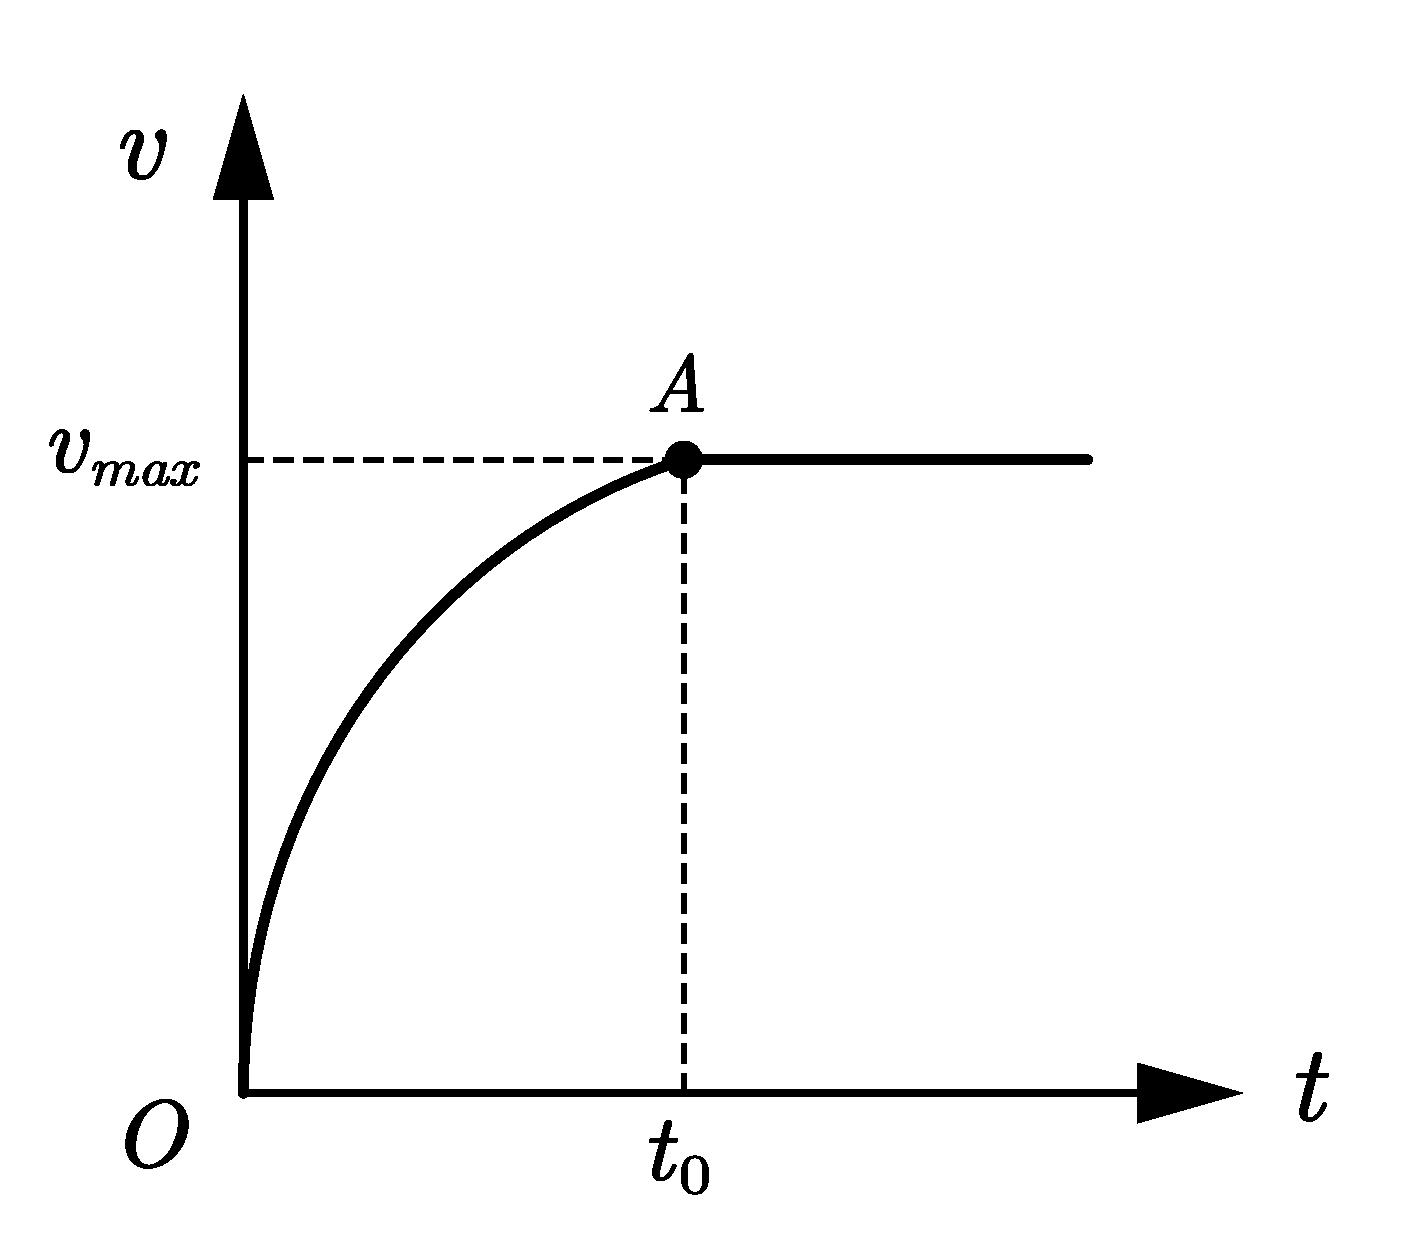
\includegraphics[width=0.31\textwidth]{pic/pic10.pdf}
	\label{fic10}
\end{wrapfigure}
由此解得
\begin{equation}
	v_\mathrm{max} = \frac{P}{F_\mathrm{f}}.
	\label{最大速度}
\end{equation}
由(\ref{恒定功率启动的牛二律})可知, 当机车的牵引力$F$与所受阻力$F_\mathrm{f}$相等时, 机车速度达到最大值$v_\mathrm{max}$.

右图是质量为$m$的机车以恒定功率$P$启动的$v-t$图像. 在$OA$段, 机车的加速度逐渐减小;
在$A$点处, 机车的加速度降为0, 机车的牵引力$F$等于阻力$F_\mathrm{f}$.

如何求出机车的位移呢? 因为机车做的不是匀变速直线运动, 我们没有直接的公式可以计算;
$v - t$图线与坐标轴围成的图形也不规则, 不易计算面积. 我们不妨试试刚学的动能定理.
根据动能定理, 机车的牵引力做功与所受阻力做功的代数和等于机车动能的变化量, 即
$$Pt_0 - F_\mathrm{f}x = \frac12 m v_\mathrm{max}^2 - 0.$$
由此即可解出机车的位移$x$.

\subsubsection*{恒定加速度的机车启动问题}

\begin{wrapfigure}{r}{5cm}
	\flushright
	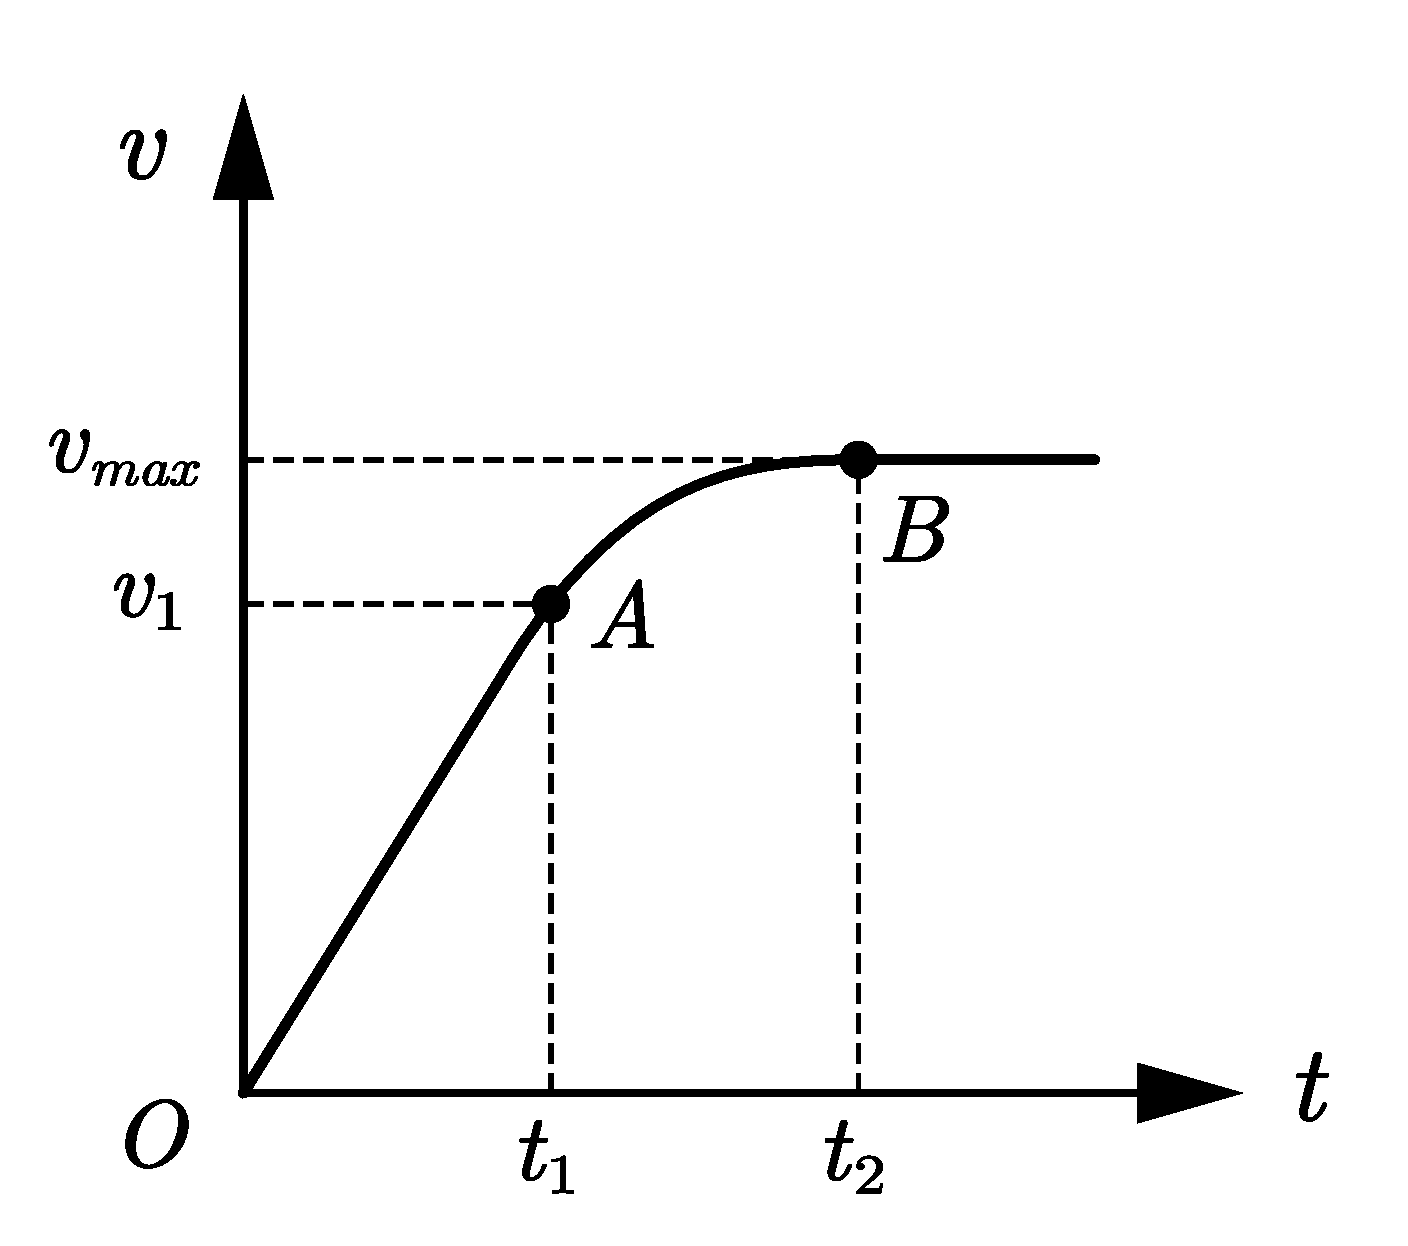
\includegraphics[width=0.31\textwidth]{pic/pic11.pdf}
	\label{fic11}
\end{wrapfigure}

当机车以恒定加速度$a$启动时, 机车的速率$v$持续增加. 因为合力$ma = F - F_\mathrm{f}$, 且
阻力$F_\mathrm{f}$是定值, 所以当加速度恒定时, 牵引力$F$也是恒定的. 根据(\ref{机车启动功率}),
机车的瞬时功率也持续增加. 由于机车有额定功率$P_\mathrm{max}$, 因此机车以恒定加速度
启动时, 最终一定会达到最大功率$P_\mathrm{max}$, \textbf{从而也会进入恒定功率的状态}.

右图是质量为$m$的机车以恒定加速度$a$启动的$v-t$图像, 直线$OA$是机车以加速度$a$做
匀加速直线运动的$v-t$图线, 其牵引力$F$恒定不变; 在$A$点处, 机车达到额定功率$P_\mathrm{max}$.
机车的匀加速运动结束于$A$点, 此时机车的速率为$v_1$, 类似(\ref{机车启动牛二律})(\ref{机车启动功率})有
$$F_1 - F_\mathrm{f} = ma,$$ $$P_\mathrm{max} = F_1v_1.$$
由此解得$$v_1 = \frac{P_\mathrm{max}}{ma+F_\mathrm{f}}.$$
再根据$v_1 = at_1$, 可以求出$t_1$.

曲线$AB$是机车以额定功率$P_\mathrm{max}$继续运动的$v-t$图线, 因为汽车的速率继续增大, 根据(\ref{机车启动功率}),
机车的牵引力逐渐减小; 在点$B$处, 机车的加速度降为0, 机车的牵引力$F$等于阻力$F_\mathrm{f}$,
机车达到最大速度$v_\mathrm{max}$. 类似(\ref{最大速度}), 容易知道$$v_\mathrm{max} = \frac{P_\mathrm{max}}{F_\mathrm{f}}.$$

\subsection{机械能守恒定律}

力做功的过程, 也是能量从一种形式转化为另一种形式的过程.在初中时我们就知道, 在一定条件下, 物体的动能和势能
可以相互转化.

我们把物体的动能和势能统称为\textbf{物体的机械能}. 如果这个物体是弹簧, 那么它有动能, 重力势能和弹性势能
三种机械能; 而刚性的物体只有动能, 重力势能两种机械能\footnote{事实上, 任何物体在力的作用下都会发生弹性形变,
	而除弹簧外, 大部分物体发生的形变是肉眼不可见的, 即形变量极小, 在宏观上我们忽略不计.}.

\subparagraph{单个物体的机械能守恒} \textbf{只有重力做功的物体, 它的动能和重力势能可以互相转化, 但它们的总和
	保持不变, 即这个物体的机械能守恒.}

\subparagraph{系统的机械能守恒}\textbf{在只有重力和弹力做功的物体系统中, 系统的动能和势能可以互相转化,
	而它们的总和保持不变}.这就是\textbf{机械能守恒定律}.它可以表示为
$$E_\mathrm{k1}+E_\mathrm{p1} = E_\mathrm{k2} = E_\mathrm{p2}.$$

需要注意的是, 在多个物体组成的物体系统中, 即使该系统不受其它外力作用,
单个物体的机械能也不一定守恒, 但该系统内所有物体的的机械能总和一定守恒.

如果一个物体系统除了重力和系统内力(即各物体间的弹力)外还有其它力做功, 那么该系统的机械能不守恒,
并且``其它力''做的功等于该系统机械能的变化量.如果用$\Delta E_\mathrm{m}$表示机械能的变化量, 用$W_\text{其它}$
表示``其它力''做功,那么上述内容可以表示为$$W_\text{其它}= \Delta E_\mathrm{m}.$$

\begin{wrapfigure}{r}{5cm}
	\flushright
	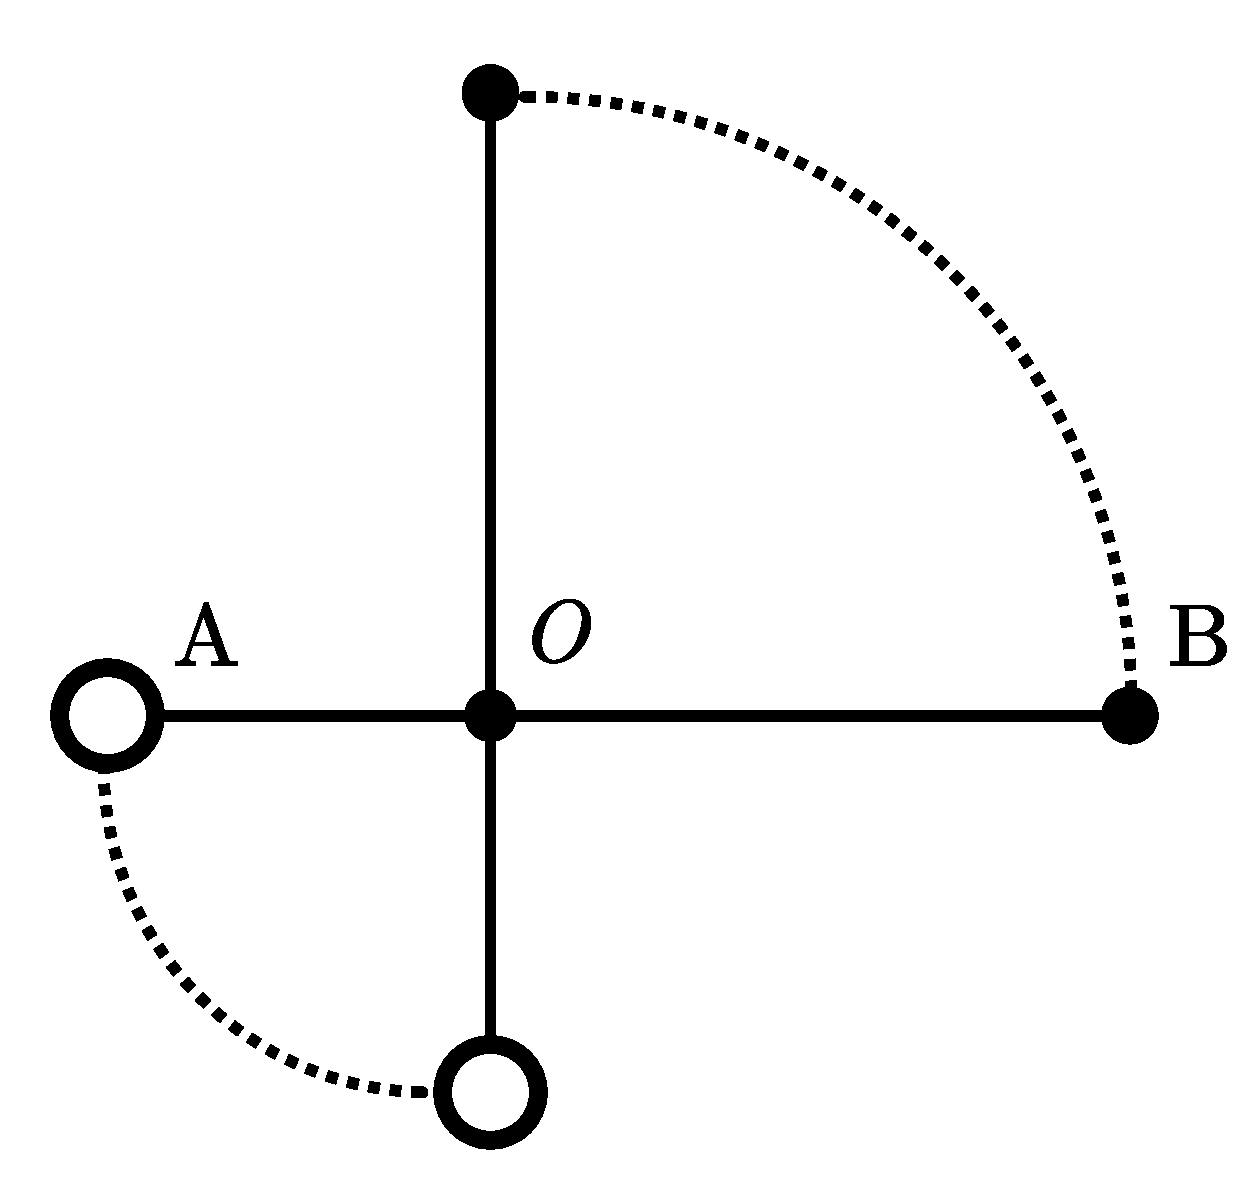
\includegraphics[width=0.3\textwidth]{pic/exam_5.6-2.pdf}
	\label{fic13}
\end{wrapfigure}

\refstepcounter{exam}
\subparagraph{例\theexam}如图所示, A, B 两小球分别固定在一刚性轻杆的两端, 两球球心间相距$L$, 两球质量分别为$m_A = 4.0\ \mathrm{kg}$,
$m_B = 1.0\ \mathrm{kg}$,
杆上距A球球心$0.4L$处有一水平轴$O$, 杆可绕轴无摩擦转动. 现先使杆保持水平, 然后从静止释放. 当杆转到竖直位置时, 求:

(1)当杆转到竖直位置时两球的速度$v_\mathrm{A}$, $v_\mathrm{B}$;

(2)杆对A球的作用力$F$;

(3)转动过程中杆对A球做的功$W$.

\textbf{解}\ \ \ (1) 由圆周运动的知识可知, A, B 两小球运动的角速度相等.设它们到轴$O$的距离分别为$L_\mathrm{A}$,
$L_\mathrm{B}$, 根据线速度与加速度的关系有$$\frac{v_\mathrm{A}}{v_\mathrm{B}} = \frac{L_\mathrm{A}}{L_\mathrm{B}}.$$
\setlength{\abovedisplayskip}{5pt}
\setlength{\belowdisplayskip}{10pt}

取杆的初位置为重力势能的参考平面, 以两球组成的系统为研究对象, 由机械能守恒定律得
$$-m_\mathrm{A}gL_\mathrm{A}+m_\mathrm{B}gL_\mathrm{B} = \frac12 m_\mathrm{A} v_\mathrm{A}^2 + \frac12 m_\mathrm{B}v_\mathrm{B}^2.$$

联立解得$v_\mathrm{A} = \displaystyle\frac{4\sqrt{5}}{5}\ \mathrm{m/s}$
, $v_\mathrm{B} = \displaystyle\frac{6\sqrt{5}}{5}\ \mathrm{m/s}$.

\setlength{\abovedisplayskip}{3pt}
\setlength{\belowdisplayskip}{3pt}

(2) 对小球A应用牛顿第二定律得
$$F - m_\mathrm{A}g = m_\mathrm{A}\frac{v_\mathrm{A}^2}{L_\mathrm{A}}.$$
由此可得$F= 72$\ N.

(3) 对A应用动能定理得$$m_\mathrm{A}gL_\mathrm{A} + W = \frac12 m_\mathrm{A}v^2_\mathrm{A}.$$
由此解得$W = -9.6$\ J.

\subsection{能量的守恒与转化}

\subsubsection{功与能的关系}

不同形式的能量之间的转化通过做功来实现, 即做功的过程
是能量转化的过程. 物体做了多少功, 就有多少能量发生了转化, 而
功的正负表示能量的转化方向(即增加与减少).因此, \textbf{功是能量转化的量度}.

\subsubsection{摩擦生热}

两个粗糙的物体发生$\Delta x$的相对滑动, 如果它们之间的滑动摩擦力做功为$W_\mathrm{f}$, 那么
该过程产生的热量为$$Q = W_\mathrm{f} \cdot \Delta x.$$

因为摩擦力是重力和弹力之外的``其他力'', 所以当有摩擦力做功时, 机械能不守恒. 事实上, 机械能
转化为了热量$Q$, 这就是\textbf{摩擦生热}.

\subsubsection{能量守恒}

\subparagraph{能量守恒定律} 能量既不会凭空产生, 也不会凭空消失, 它只会从一种形式转化为另一种形式,
或者从一个物体转移到另一个物体, 而在转移或转化的过程中, 能量的总量保持不变.

能量守恒定律告诉我们:\textbf{某种形式的能量减少, 一定存在其他形式的能量增加; 某个物体的
	能量减少, 一定存在其他物体的能量增加. 增加量和减少量一定相等.}

这启示我们可以利用初时刻总能量等于末时刻总能量列式, 或者通过能量的增加量等于能量的减少量
列式. 应用能量守恒定律的关键是分析清楚系统中有哪几种形式的能量, 发生了哪些转化或转移过程.\\

把一个物块轻放在恒定速度运转的水平传送带上, 假设传送带足够长, 物块将持续加速, 最终与传送带共速,
它的动能是从哪里来的呢? 如果是倾斜的传送带, 物块从传送带的最低点升至最高点, 那么物块的重力势能又
是从何而来的呢?

事实上, 物块随传送带运动时传送带的耗电量, 是比传送带自己转动时的耗电量更多的. 传送带自己转动时,电能转化为了
焦耳热和传送带机械内部的摩擦生热;当物块被放在传送带上时, 电能还转化为物块的机械能以及物块与传送带的摩擦生热.
因此, 根据能量守恒定律, 传送带多消耗的电能为
$$\Delta E_\text{电} = Q + \Delta E_\text{物块},$$
式中$\Delta E_\text{电}$是传送带多消耗的电能, $\Delta E_\text{物块}$是
物块机械能的变化量, $Q$是物块与传送带的摩擦生热, 等于物块受到的摩擦力乘以物块与传送带的相对位移.


\begin{wrapfigure}{r}{6cm}
	\flushright
	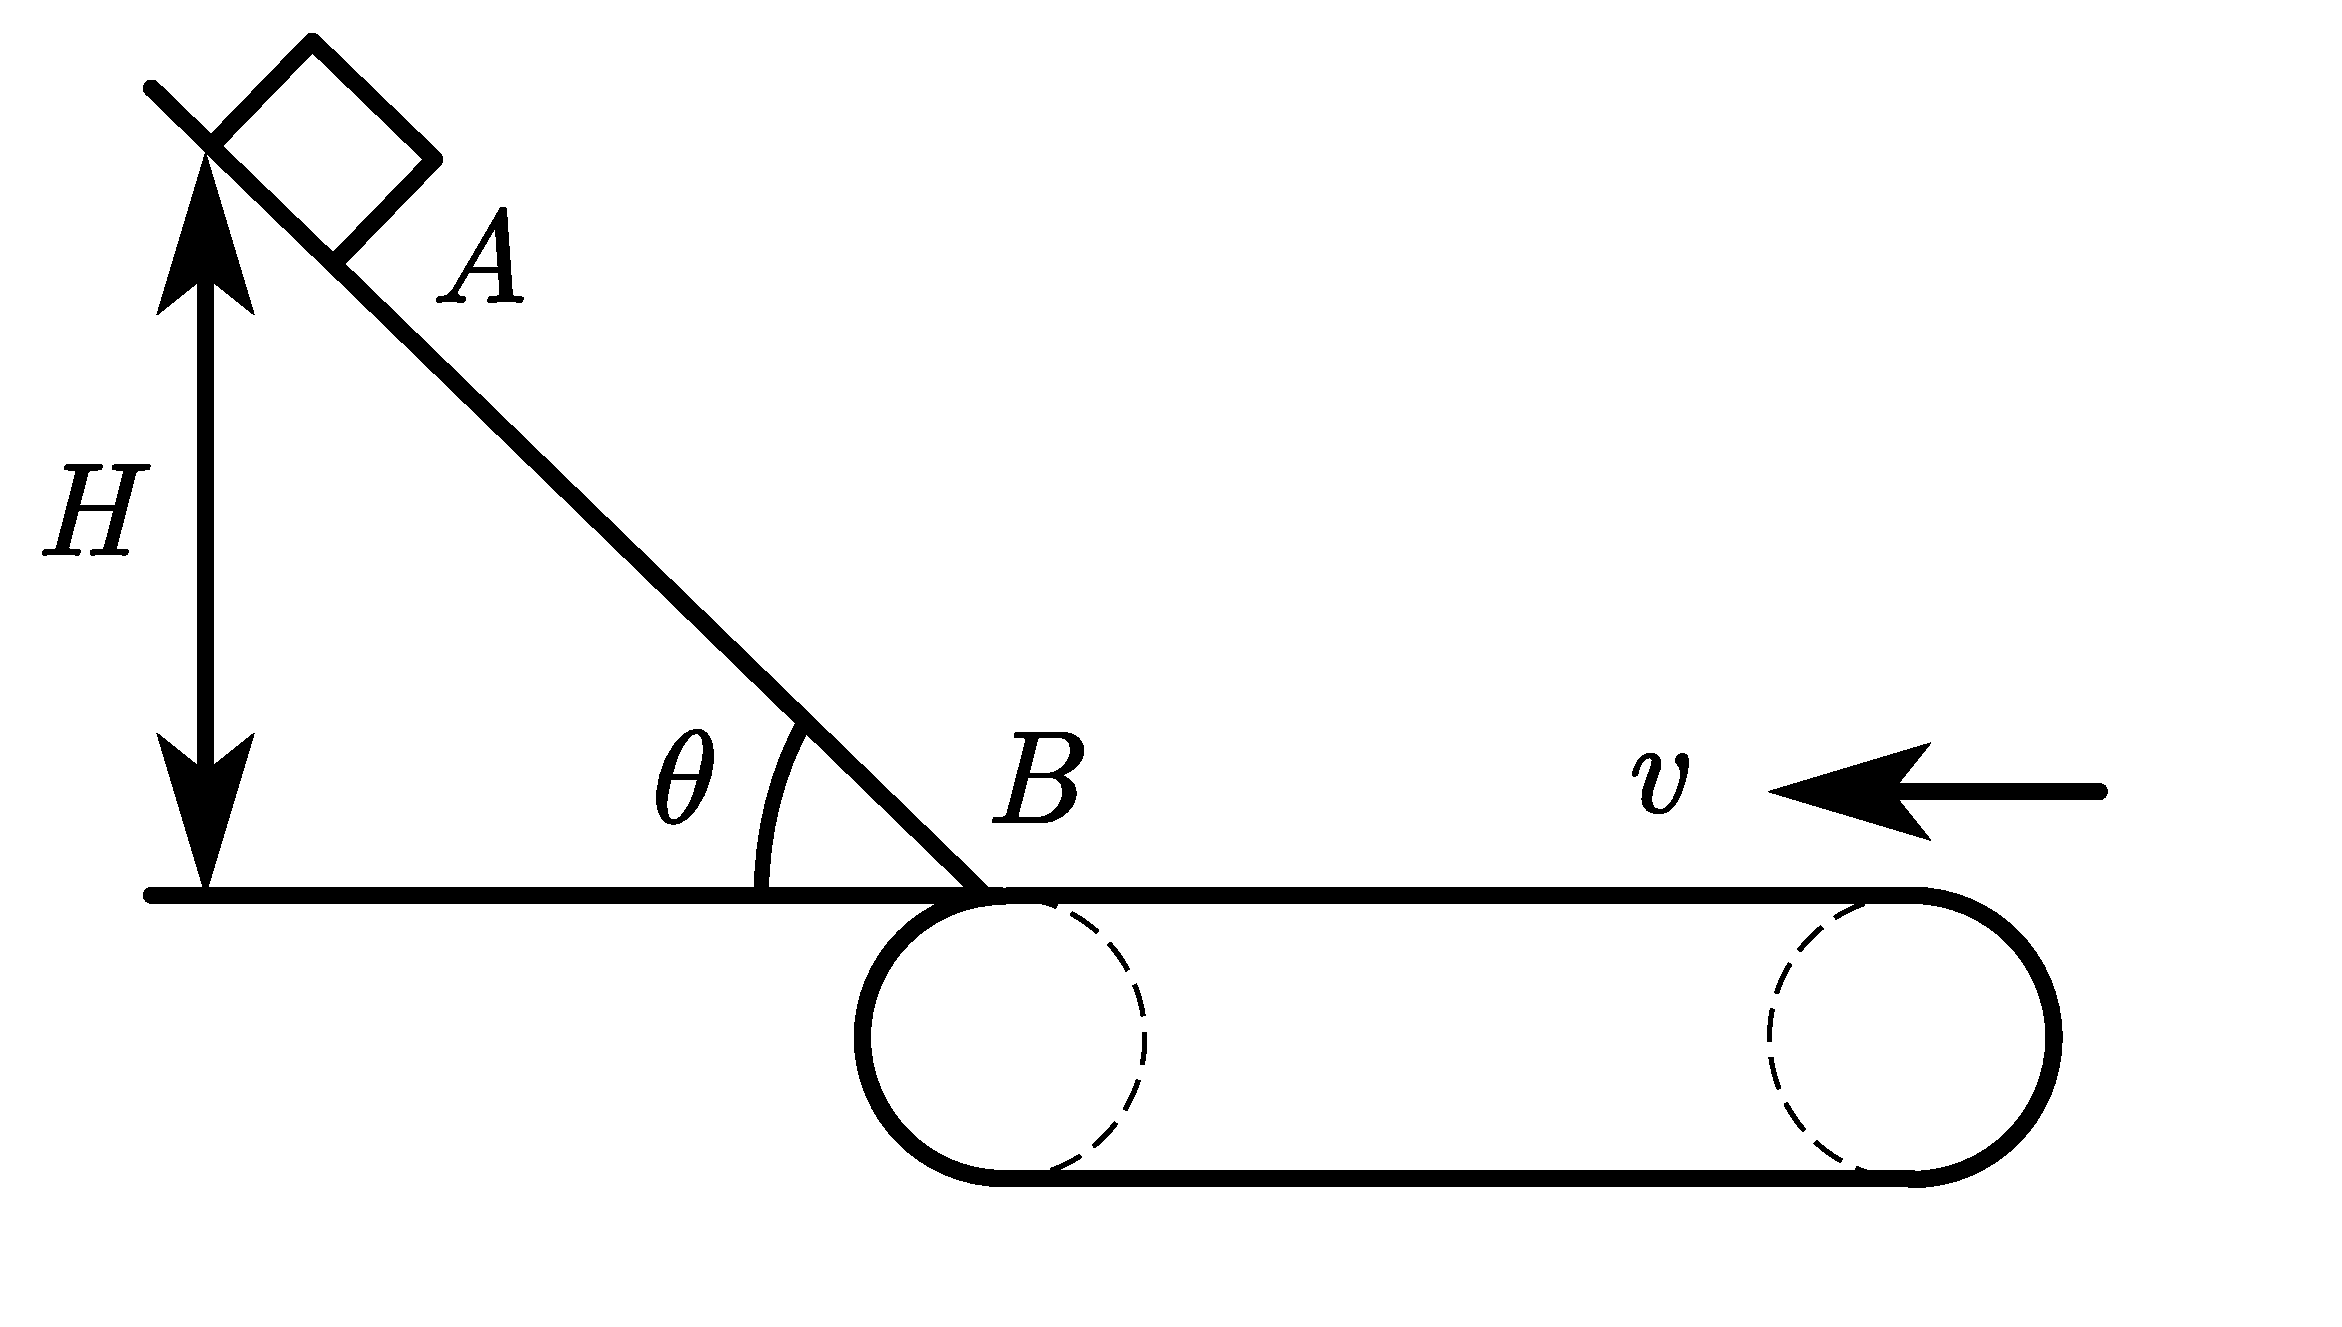
\includegraphics[width=0.4\textwidth]{pic/exam_5-3.pdf}
	\label{fic14}
\end{wrapfigure}
\refstepcounter{exam}
\subparagraph{例\theexam} 如图所示, 倾角$\theta = 37^{\circ}$的斜面与足够长的水平传送带相连接(接口处平滑)
, 传送带逆时针转动, 速度$v = 6\ \mathrm{m/s}$.某时刻质量$m = 1\ \mathrm{kg}$的物块(可视为质点)
从斜面上距离传送带水平面高$H = 3\ \mathrm{m}$处的$A$点由静止滑下.物块与传送带和物块与斜面间的动摩擦
因数均为$\mu = 0.3$. 已知$\sin 37^{\circ} = 0.6, \cos 37^{\circ} = 0.8$, 重力加速度$g$取$10\ \mathrm{m/s^2}$.
求物块在传送带上第一次相对地面静止时, 由于物块滑上传送带而使传送带多做的功$\Delta W$.

\textbf{解}\ \ \ 设物块运动到$B$点时速度为$v_B$, 应用动能定理得
\begin{equation*}
	mgH - \mu mg\cos \theta \ \frac{H}{\sin \theta} = \frac12 mv^2_B-0.
	\tag{i}
	\setlength{\abovedisplayskip}{5pt}
	\setlength{\belowdisplayskip}{10pt}
\end{equation*}

根据能量守恒定律, 从物块到达$B$点到物块第一次相对地面静止, 物块的动能$E_\mathrm{k} = \displaystyle\frac12 m v_B^2$
以及传送带多做的功$\Delta W$,
都转化为物块与传送带的摩擦生热$Q = \mu mg\Delta s$, 即
\begin{equation*}
	\frac12 m v_B^2 + \Delta W = \mu mg \Delta s,
	\setlength{\abovedisplayskip}{5pt}
	\setlength{\belowdisplayskip}{5pt}
	\tag{ii}
\end{equation*}
其中$\Delta s$是物块与传送带的相对位移.

物块在传送带上做匀减速运动, 有
\setlength{\abovedisplayskip}{0pt}
\setlength{\belowdisplayskip}{0pt}
\begin{equation*}
	-\mu mg = ma,
	\tag{iii}
\end{equation*}
\begin{equation*}
	0 = v_B-at.
	\tag{iv}
\end{equation*}

物块相对地面的位移
\begin{equation*}
	s_1 = v_Bt-\frac12 at^2,
	\tag{v}
\end{equation*}
传送带在这段过程中相对地面的位移
\begin{equation*}
	s_2 = vt.
	\tag{vi}
\end{equation*}
因为物块和传送带在这段过程中是反向运动的, 所以它们的相对位移
\begin{equation*}
	\Delta s = s_1 + s_2.
	\tag{vii}
\end{equation*}

由此解出$\Delta W = 36\ \mathrm{J}$.

\end{document}